% Options for packages loaded elsewhere
% Options for packages loaded elsewhere
\PassOptionsToPackage{unicode}{hyperref}
\PassOptionsToPackage{hyphens}{url}
\PassOptionsToPackage{dvipsnames,svgnames,x11names}{xcolor}
%
\documentclass[
  spanish,
  11pt,
  letterpaper,
]{book}
\usepackage{xcolor}
\usepackage[margin=2.3cm]{geometry}
\usepackage{amsmath,amssymb}
\setcounter{secnumdepth}{5}
\usepackage{iftex}
\ifPDFTeX
  \usepackage[T1]{fontenc}
  \usepackage[utf8]{inputenc}
  \usepackage{textcomp} % provide euro and other symbols
\else % if luatex or xetex
  \usepackage{unicode-math} % this also loads fontspec
  \defaultfontfeatures{Scale=MatchLowercase}
  \defaultfontfeatures[\rmfamily]{Ligatures=TeX,Scale=1}
\fi
\usepackage{lmodern}
\ifPDFTeX\else
  % xetex/luatex font selection
\fi
% Use upquote if available, for straight quotes in verbatim environments
\IfFileExists{upquote.sty}{\usepackage{upquote}}{}
\IfFileExists{microtype.sty}{% use microtype if available
  \usepackage[]{microtype}
  \UseMicrotypeSet[protrusion]{basicmath} % disable protrusion for tt fonts
}{}
\makeatletter
\@ifundefined{KOMAClassName}{% if non-KOMA class
  \IfFileExists{parskip.sty}{%
    \usepackage{parskip}
  }{% else
    \setlength{\parindent}{0pt}
    \setlength{\parskip}{6pt plus 2pt minus 1pt}}
}{% if KOMA class
  \KOMAoptions{parskip=half}}
\makeatother
% Make \paragraph and \subparagraph free-standing
\makeatletter
\ifx\paragraph\undefined\else
  \let\oldparagraph\paragraph
  \renewcommand{\paragraph}{
    \@ifstar
      \xxxParagraphStar
      \xxxParagraphNoStar
  }
  \newcommand{\xxxParagraphStar}[1]{\oldparagraph*{#1}\mbox{}}
  \newcommand{\xxxParagraphNoStar}[1]{\oldparagraph{#1}\mbox{}}
\fi
\ifx\subparagraph\undefined\else
  \let\oldsubparagraph\subparagraph
  \renewcommand{\subparagraph}{
    \@ifstar
      \xxxSubParagraphStar
      \xxxSubParagraphNoStar
  }
  \newcommand{\xxxSubParagraphStar}[1]{\oldsubparagraph*{#1}\mbox{}}
  \newcommand{\xxxSubParagraphNoStar}[1]{\oldsubparagraph{#1}\mbox{}}
\fi
\makeatother

\usepackage{color}
\usepackage{fancyvrb}
\newcommand{\VerbBar}{|}
\newcommand{\VERB}{\Verb[commandchars=\\\{\}]}
\DefineVerbatimEnvironment{Highlighting}{Verbatim}{commandchars=\\\{\}}
% Add ',fontsize=\small' for more characters per line
\newenvironment{Shaded}{}{}
\newcommand{\AlertTok}[1]{\textcolor[rgb]{1.00,0.33,0.33}{\textbf{#1}}}
\newcommand{\AnnotationTok}[1]{\textcolor[rgb]{0.42,0.45,0.49}{#1}}
\newcommand{\AttributeTok}[1]{\textcolor[rgb]{0.84,0.23,0.29}{#1}}
\newcommand{\BaseNTok}[1]{\textcolor[rgb]{0.00,0.36,0.77}{#1}}
\newcommand{\BuiltInTok}[1]{\textcolor[rgb]{0.84,0.23,0.29}{#1}}
\newcommand{\CharTok}[1]{\textcolor[rgb]{0.01,0.18,0.38}{#1}}
\newcommand{\CommentTok}[1]{\textcolor[rgb]{0.42,0.45,0.49}{#1}}
\newcommand{\CommentVarTok}[1]{\textcolor[rgb]{0.42,0.45,0.49}{#1}}
\newcommand{\ConstantTok}[1]{\textcolor[rgb]{0.00,0.36,0.77}{#1}}
\newcommand{\ControlFlowTok}[1]{\textcolor[rgb]{0.84,0.23,0.29}{#1}}
\newcommand{\DataTypeTok}[1]{\textcolor[rgb]{0.84,0.23,0.29}{#1}}
\newcommand{\DecValTok}[1]{\textcolor[rgb]{0.00,0.36,0.77}{#1}}
\newcommand{\DocumentationTok}[1]{\textcolor[rgb]{0.42,0.45,0.49}{#1}}
\newcommand{\ErrorTok}[1]{\textcolor[rgb]{1.00,0.33,0.33}{\underline{#1}}}
\newcommand{\ExtensionTok}[1]{\textcolor[rgb]{0.84,0.23,0.29}{\textbf{#1}}}
\newcommand{\FloatTok}[1]{\textcolor[rgb]{0.00,0.36,0.77}{#1}}
\newcommand{\FunctionTok}[1]{\textcolor[rgb]{0.44,0.26,0.76}{#1}}
\newcommand{\ImportTok}[1]{\textcolor[rgb]{0.01,0.18,0.38}{#1}}
\newcommand{\InformationTok}[1]{\textcolor[rgb]{0.42,0.45,0.49}{#1}}
\newcommand{\KeywordTok}[1]{\textcolor[rgb]{0.84,0.23,0.29}{#1}}
\newcommand{\NormalTok}[1]{\textcolor[rgb]{0.14,0.16,0.18}{#1}}
\newcommand{\OperatorTok}[1]{\textcolor[rgb]{0.14,0.16,0.18}{#1}}
\newcommand{\OtherTok}[1]{\textcolor[rgb]{0.44,0.26,0.76}{#1}}
\newcommand{\PreprocessorTok}[1]{\textcolor[rgb]{0.84,0.23,0.29}{#1}}
\newcommand{\RegionMarkerTok}[1]{\textcolor[rgb]{0.42,0.45,0.49}{#1}}
\newcommand{\SpecialCharTok}[1]{\textcolor[rgb]{0.00,0.36,0.77}{#1}}
\newcommand{\SpecialStringTok}[1]{\textcolor[rgb]{0.01,0.18,0.38}{#1}}
\newcommand{\StringTok}[1]{\textcolor[rgb]{0.01,0.18,0.38}{#1}}
\newcommand{\VariableTok}[1]{\textcolor[rgb]{0.89,0.38,0.04}{#1}}
\newcommand{\VerbatimStringTok}[1]{\textcolor[rgb]{0.01,0.18,0.38}{#1}}
\newcommand{\WarningTok}[1]{\textcolor[rgb]{1.00,0.33,0.33}{#1}}

\usepackage{longtable,booktabs,array}
\newcounter{none} % for unnumbered tables
\usepackage{calc} % for calculating minipage widths
% Correct order of tables after \paragraph or \subparagraph
\usepackage{etoolbox}
\makeatletter
\patchcmd\longtable{\par}{\if@noskipsec\mbox{}\fi\par}{}{}
\makeatother
% Allow footnotes in longtable head/foot
\IfFileExists{footnotehyper.sty}{\usepackage{footnotehyper}}{\usepackage{footnote}}
\makesavenoteenv{longtable}
\usepackage{graphicx}
\makeatletter
\newsavebox\pandoc@box
\newcommand*\pandocbounded[1]{% scales image to fit in text height/width
  \sbox\pandoc@box{#1}%
  \Gscale@div\@tempa{\textheight}{\dimexpr\ht\pandoc@box+\dp\pandoc@box\relax}%
  \Gscale@div\@tempb{\linewidth}{\wd\pandoc@box}%
  \ifdim\@tempb\p@<\@tempa\p@\let\@tempa\@tempb\fi% select the smaller of both
  \ifdim\@tempa\p@<\p@\scalebox{\@tempa}{\usebox\pandoc@box}%
  \else\usebox{\pandoc@box}%
  \fi%
}
% Set default figure placement to htbp
\def\fps@figure{htbp}
\makeatother



\ifLuaTeX
\usepackage[bidi=basic,shorthands=off]{babel}
\else
\usepackage[bidi=default,shorthands=off]{babel}
\fi
\ifLuaTeX
  \usepackage{selnolig} % disable illegal ligatures
\fi


\setlength{\emergencystretch}{3em} % prevent overfull lines

\providecommand{\tightlist}{%
  \setlength{\itemsep}{0pt}\setlength{\parskip}{0pt}}



 


\usepackage{xcolor}
\usepackage{fvextra}
\usepackage{tcolorbox}
\usepackage{titlesec}
\usepackage{fontspec}
\definecolor{azulLibro}{HTML}{1F4E79}
\definecolor{turquesaLibro}{HTML}{19A7AE}
\definecolor{grisCodigo}{HTML}{F3F6FA}
\definecolor{bordeCodigo}{HTML}{B7C7D9}
\definecolor{coralLibro}{HTML}{D95D39}
\fvset{breaklines=true,breakanywhere=true,fontsize=\scriptsize,frame=single,framesep=2mm,rulecolor=\color{bordeCodigo},baselinestretch=1.02}
\titleformat{\chapter}[display]
  {\normalfont\Huge\bfseries\color{azulLibro}}
  {\chaptertitlename\ \thechapter}{12pt}{\Huge}
\titleformat{\section}
  {\normalfont\Large\bfseries\color{azulLibro}}
  {\thesection}{0.8em}{}
\titleformat{\subsection}
  {\normalfont\large\bfseries\color{turquesaLibro}}
  {\thesubsection}{0.8em}{}
\renewcommand{\contentsname}{Índice general}
\renewcommand{\chaptername}{Capítulo}
\makeatletter
\@ifpackageloaded{tcolorbox}{}{\usepackage[skins,breakable]{tcolorbox}}
\@ifpackageloaded{fontawesome5}{}{\usepackage{fontawesome5}}
\definecolor{quarto-callout-color}{HTML}{909090}
\definecolor{quarto-callout-note-color}{HTML}{0758E5}
\definecolor{quarto-callout-important-color}{HTML}{CC1914}
\definecolor{quarto-callout-warning-color}{HTML}{EB9113}
\definecolor{quarto-callout-tip-color}{HTML}{00A047}
\definecolor{quarto-callout-caution-color}{HTML}{FC5300}
\definecolor{quarto-callout-color-frame}{HTML}{acacac}
\definecolor{quarto-callout-note-color-frame}{HTML}{4582ec}
\definecolor{quarto-callout-important-color-frame}{HTML}{d9534f}
\definecolor{quarto-callout-warning-color-frame}{HTML}{f0ad4e}
\definecolor{quarto-callout-tip-color-frame}{HTML}{02b875}
\definecolor{quarto-callout-caution-color-frame}{HTML}{fd7e14}
\makeatother
\makeatletter
\@ifpackageloaded{bookmark}{}{\usepackage{bookmark}}
\makeatother
\makeatletter
\@ifpackageloaded{caption}{}{\usepackage{caption}}
\AtBeginDocument{%
\ifdefined\contentsname
  \renewcommand*\contentsname{Tabla de contenidos}
\else
  \newcommand\contentsname{Tabla de contenidos}
\fi
\ifdefined\listfigurename
  \renewcommand*\listfigurename{Listado de Figuras}
\else
  \newcommand\listfigurename{Listado de Figuras}
\fi
\ifdefined\listtablename
  \renewcommand*\listtablename{Listado de Tablas}
\else
  \newcommand\listtablename{Listado de Tablas}
\fi
\ifdefined\figurename
  \renewcommand*\figurename{Figura}
\else
  \newcommand\figurename{Figura}
\fi
\ifdefined\tablename
  \renewcommand*\tablename{Tabla}
\else
  \newcommand\tablename{Tabla}
\fi
}
\@ifpackageloaded{float}{}{\usepackage{float}}
\floatstyle{ruled}
\@ifundefined{c@chapter}{\newfloat{codelisting}{h}{lop}}{\newfloat{codelisting}{h}{lop}[chapter]}
\floatname{codelisting}{Listado}
\newcommand*\listoflistings{\listof{codelisting}{Listado de Listados}}
\makeatother
\makeatletter
\makeatother
\makeatletter
\@ifpackageloaded{caption}{}{\usepackage{caption}}
\@ifpackageloaded{subcaption}{}{\usepackage{subcaption}}
\makeatother
\usepackage{bookmark}
\IfFileExists{xurl.sty}{\usepackage{xurl}}{} % add URL line breaks if available
\urlstyle{same}
\hypersetup{
  pdftitle={Aprendizaje y Clasificación Automática con R},
  pdfauthor={MI Jesús Gilberto Rodríguez Escobedo},
  pdflang={es},
  colorlinks=true,
  linkcolor={Maroon},
  filecolor={Maroon},
  citecolor={Blue},
  urlcolor={Blue},
  pdfcreator={LaTeX via pandoc}}


\title{Aprendizaje y Clasificación Automática con R}
\usepackage{etoolbox}
\makeatletter
\providecommand{\subtitle}[1]{% add subtitle to \maketitle
  \apptocmd{\@title}{\par {\large #1 \par}}{}{}
}
\makeatother
\subtitle{Un enfoque práctico con datos abiertos reales}
\author{MI Jesús Gilberto Rodríguez Escobedo}
\date{2026-07-10}
\begin{document}
\frontmatter
\maketitle

\renewcommand*\contentsname{Índice general}
{
\setcounter{tocdepth}{2}
\tableofcontents
}

\mainmatter
\bookmarksetup{startatroot}

\chapter*{Presentación}\label{presentaciuxf3n}
\addcontentsline{toc}{chapter}{Presentación}

\markboth{Presentación}{Presentación}

\section*{Aprendizaje y Clasificación Automática con
R}\label{aprendizaje-y-clasificaciuxf3n-automuxe1tica-con-r}
\addcontentsline{toc}{section}{Aprendizaje y Clasificación Automática
con R}

\markright{Aprendizaje y Clasificación Automática con R}

\subsection*{Un enfoque práctico con datos abiertos
reales}\label{un-enfoque-pruxe1ctico-con-datos-abiertos-reales}
\addcontentsline{toc}{subsection}{Un enfoque práctico con datos abiertos
reales}

\textbf{Autor:} MI Jesús Gilberto Rodríguez Escobedo\\
\textbf{Versión:} 0.6\\
\textbf{Modalidad:} Libro abierto, práctico e interactivo\\
\textbf{Tecnologías:} R · Quarto · Machine Learning · Datos abiertos ·
GitHub Pages

Este libro introduce el aprendizaje automático (\emph{Machine Learning})
mediante ejemplos claros, didácticos y prácticos desarrollados
principalmente en \textbf{R}.

La intención no es escribir un tratado matemático extenso, sino
construir una guía aplicada para aprender haciendo con datos abiertos
reales. En esta versión trabajamos con datos de accidentes de tránsito
de México y los usamos como hilo conductor para explicar preparación de
datos, análisis exploratorio y modelos de clasificación.

\begin{tcolorbox}[enhanced jigsaw, arc=.35mm, bottomrule=.15mm, bottomtitle=1mm, breakable, colback=white, colbacktitle=quarto-callout-note-color!10!white, colframe=quarto-callout-note-color-frame, coltitle=black, left=2mm, leftrule=.75mm, opacityback=0, opacitybacktitle=0.6, rightrule=.15mm, title=\textcolor{quarto-callout-note-color}{\faInfo}\hspace{0.5em}{Enfoque del libro}, titlerule=0mm, toprule=.15mm, toptitle=1mm]

El libro combina fundamento conceptual, código reproducible en R,
explicación breve del código, interpretación didáctica de resultados y
visualizaciones profesionales.

\end{tcolorbox}

\section*{Objetivo general}\label{objetivo-general}
\addcontentsline{toc}{section}{Objetivo general}

\markright{Objetivo general}

Desarrollar competencias básicas e intermedias en aprendizaje automático
mediante el análisis, modelado e interpretación de datos reales.

\section*{Público al que va
dirigido}\label{puxfablico-al-que-va-dirigido}
\addcontentsline{toc}{section}{Público al que va dirigido}

\markright{Público al que va dirigido}

Este libro está dirigido a estudiantes de ingeniería, ciencias, ciencia
de datos, estadística aplicada y áreas afines que desean iniciar en
aprendizaje automático con un enfoque práctico.

\section*{Software utilizado}\label{software-utilizado}
\addcontentsline{toc}{section}{Software utilizado}

\markright{Software utilizado}

\begin{itemize}
\tightlist
\item
  RStudio
\item
  Consola de R
\item
  Google Colab
\item
  GitHub
\item
  GitHub Pages
\item
  Quarto Pub
\end{itemize}

\section*{Estructura actual del
libro}\label{estructura-actual-del-libro}
\addcontentsline{toc}{section}{Estructura actual del libro}

\markright{Estructura actual del libro}

\begin{enumerate}
\def\labelenumi{\arabic{enumi}.}
\tightlist
\item
  Introducción al aprendizaje automático.
\item
  Preparación de datos reales.
\item
  Análisis exploratorio de datos.
\item
  Regresión logística.
\item
  k vecinos más cercanos.
\item
  Árboles de decisión.
\item
  Random Forest.
\end{enumerate}

\section*{Nota para el lector}\label{nota-para-el-lector}
\addcontentsline{toc}{section}{Nota para el lector}

\markright{Nota para el lector}

Los capítulos están diseñados para leerse y ejecutarse paso a paso. Cada
bloque de código busca responder una pregunta concreta y cada resultado
se acompaña de una interpretación didáctica.

\bookmarksetup{startatroot}

\chapter*{Licencia, autoría y forma de
citar}\label{licencia-autoruxeda-y-forma-de-citar}
\addcontentsline{toc}{chapter}{Licencia, autoría y forma de citar}

\markboth{Licencia, autoría y forma de citar}{Licencia, autoría y forma
de citar}

\section*{Autor}\label{autor}
\addcontentsline{toc}{section}{Autor}

\markright{Autor}

\textbf{MI Jesús Gilberto Rodríguez Escobedo}

\section*{Licencia}\label{licencia}
\addcontentsline{toc}{section}{Licencia}

\markright{Licencia}

Este libro se distribuye bajo la licencia \textbf{Creative Commons
Atribución-NoComercial-CompartirIgual 4.0 Internacional (CC BY-NC-SA
4.0)}.

Esto significa que el material puede compartirse y adaptarse con fines
educativos y no comerciales, siempre que se otorgue el crédito
correspondiente al autor y las obras derivadas se compartan bajo una
licencia compatible.

\section*{Cita sugerida}\label{cita-sugerida}
\addcontentsline{toc}{section}{Cita sugerida}

\markright{Cita sugerida}

Rodríguez Escobedo, J. G. (2026). \emph{Aprendizaje y Clasificación
Automática con R: Un enfoque práctico con datos abiertos reales}. Libro
web publicado con Quarto y GitHub Pages.

\section*{Uso educativo}\label{uso-educativo}
\addcontentsline{toc}{section}{Uso educativo}

\markright{Uso educativo}

El propósito de este libro es apoyar la enseñanza y el aprendizaje de
técnicas de aprendizaje automático con R, usando datos reales y un
enfoque didáctico, reproducible y aplicado.

\bookmarksetup{startatroot}

\chapter{¿Qué es el aprendizaje
automático?}\label{quuxe9-es-el-aprendizaje-automuxe1tico}

\section{Objetivos del capítulo}\label{objetivos-del-capuxedtulo}

Al finalizar este capítulo, el lector será capaz de explicar qué es el
aprendizaje automático, diferenciarlo de la programación tradicional e
identificar problemas de clasificación, regresión y agrupamiento.

\section{Introducción}\label{introducciuxf3n}

El aprendizaje automático, también conocido como \emph{Machine
Learning}, permite construir modelos capaces de aprender patrones a
partir de datos.

En la programación tradicional, una persona define reglas. En
aprendizaje automático, proporcionamos ejemplos para que un algoritmo
aprenda una relación entre variables de entrada y una salida esperada.

\section{Programación tradicional contra aprendizaje
automático}\label{programaciuxf3n-tradicional-contra-aprendizaje-automuxe1tico}

\begin{Shaded}
\begin{Highlighting}[]
\NormalTok{pm10 }\OtherTok{\textless{}{-}} \DecValTok{85}

\ControlFlowTok{if}\NormalTok{ (pm10 }\SpecialCharTok{\textgreater{}} \DecValTok{75}\NormalTok{) \{}
  \FunctionTok{print}\NormalTok{(}\StringTok{"Contaminación alta"}\NormalTok{)}
\NormalTok{\} }\ControlFlowTok{else}\NormalTok{ \{}
  \FunctionTok{print}\NormalTok{(}\StringTok{"Contaminación baja"}\NormalTok{)}
\NormalTok{\}}
\end{Highlighting}
\end{Shaded}

\begin{verbatim}
[1] "Contaminación alta"
\end{verbatim}

\begin{tcolorbox}[enhanced jigsaw, arc=.35mm, bottomrule=.15mm, bottomtitle=1mm, breakable, colback=white, colbacktitle=quarto-callout-note-color!10!white, colframe=quarto-callout-note-color-frame, coltitle=black, left=2mm, leftrule=.75mm, opacityback=0, opacitybacktitle=0.6, rightrule=.15mm, title=\textcolor{quarto-callout-note-color}{\faInfo}\hspace{0.5em}{Explicación del código}, titlerule=0mm, toprule=.15mm, toptitle=1mm]

Se define un valor de PM10 y después se aplica una regla fija. Si el
valor es mayor que 75, el programa clasifica el día como de
contaminación alta.

\end{tcolorbox}

\begin{tcolorbox}[enhanced jigsaw, arc=.35mm, bottomrule=.15mm, bottomtitle=1mm, breakable, colback=white, colbacktitle=quarto-callout-tip-color!10!white, colframe=quarto-callout-tip-color-frame, coltitle=black, left=2mm, leftrule=.75mm, opacityback=0, opacitybacktitle=0.6, rightrule=.15mm, title=\textcolor{quarto-callout-tip-color}{\faLightbulb}\hspace{0.5em}{Interpretación del resultado}, titlerule=0mm, toprule=.15mm, toptitle=1mm]

Este ejemplo representa programación tradicional: la decisión depende de
una regla escrita manualmente. En aprendizaje automático, la regla se
aprende a partir de ejemplos.

\end{tcolorbox}

\begin{Shaded}
\begin{Highlighting}[]
\NormalTok{datos }\OtherTok{\textless{}{-}} \FunctionTok{data.frame}\NormalTok{(}
  \AttributeTok{dia =} \DecValTok{1}\SpecialCharTok{:}\DecValTok{12}\NormalTok{,}
  \AttributeTok{pm10 =} \FunctionTok{c}\NormalTok{(}\DecValTok{42}\NormalTok{, }\DecValTok{88}\NormalTok{, }\DecValTok{55}\NormalTok{, }\DecValTok{120}\NormalTok{, }\DecValTok{63}\NormalTok{, }\DecValTok{95}\NormalTok{, }\DecValTok{38}\NormalTok{, }\DecValTok{110}\NormalTok{, }\DecValTok{72}\NormalTok{, }\DecValTok{130}\NormalTok{, }\DecValTok{47}\NormalTok{, }\DecValTok{99}\NormalTok{),}
  \AttributeTok{temperatura =} \FunctionTok{c}\NormalTok{(}\DecValTok{25}\NormalTok{, }\DecValTok{28}\NormalTok{, }\DecValTok{22}\NormalTok{, }\DecValTok{30}\NormalTok{, }\DecValTok{24}\NormalTok{, }\DecValTok{29}\NormalTok{, }\DecValTok{21}\NormalTok{, }\DecValTok{31}\NormalTok{, }\DecValTok{27}\NormalTok{, }\DecValTok{32}\NormalTok{, }\DecValTok{23}\NormalTok{, }\DecValTok{30}\NormalTok{),}
  \AttributeTok{humedad =} \FunctionTok{c}\NormalTok{(}\DecValTok{40}\NormalTok{, }\DecValTok{35}\NormalTok{, }\DecValTok{60}\NormalTok{, }\DecValTok{30}\NormalTok{, }\DecValTok{55}\NormalTok{, }\DecValTok{33}\NormalTok{, }\DecValTok{65}\NormalTok{, }\DecValTok{29}\NormalTok{, }\DecValTok{42}\NormalTok{, }\DecValTok{28}\NormalTok{, }\DecValTok{62}\NormalTok{, }\DecValTok{34}\NormalTok{),}
  \AttributeTok{clase =} \FunctionTok{c}\NormalTok{(}\StringTok{"Baja"}\NormalTok{, }\StringTok{"Alta"}\NormalTok{, }\StringTok{"Baja"}\NormalTok{, }\StringTok{"Alta"}\NormalTok{, }\StringTok{"Baja"}\NormalTok{, }\StringTok{"Alta"}\NormalTok{, }\StringTok{"Baja"}\NormalTok{, }\StringTok{"Alta"}\NormalTok{, }\StringTok{"Baja"}\NormalTok{, }\StringTok{"Alta"}\NormalTok{, }\StringTok{"Baja"}\NormalTok{, }\StringTok{"Alta"}\NormalTok{)}
\NormalTok{)}

\NormalTok{datos}
\end{Highlighting}
\end{Shaded}

\begin{verbatim}
   dia pm10 temperatura humedad clase
1    1   42          25      40  Baja
2    2   88          28      35  Alta
3    3   55          22      60  Baja
4    4  120          30      30  Alta
5    5   63          24      55  Baja
6    6   95          29      33  Alta
7    7   38          21      65  Baja
8    8  110          31      29  Alta
9    9   72          27      42  Baja
10  10  130          32      28  Alta
11  11   47          23      62  Baja
12  12   99          30      34  Alta
\end{verbatim}

\begin{tcolorbox}[enhanced jigsaw, arc=.35mm, bottomrule=.15mm, bottomtitle=1mm, breakable, colback=white, colbacktitle=quarto-callout-note-color!10!white, colframe=quarto-callout-note-color-frame, coltitle=black, left=2mm, leftrule=.75mm, opacityback=0, opacitybacktitle=0.6, rightrule=.15mm, title=\textcolor{quarto-callout-note-color}{\faInfo}\hspace{0.5em}{Explicación del código}, titlerule=0mm, toprule=.15mm, toptitle=1mm]

Se construye una pequeña base de datos con 12 días. Cada fila contiene
variables ambientales y una clase conocida.

\end{tcolorbox}

\section{Variables predictoras y variable
respuesta}\label{variables-predictoras-y-variable-respuesta}

La variable respuesta es la variable que queremos predecir. Las
variables predictoras son las variables que usamos como entrada para el
modelo.

\section{Tipos principales de aprendizaje
automático}\label{tipos-principales-de-aprendizaje-automuxe1tico}

\begin{enumerate}
\def\labelenumi{\arabic{enumi}.}
\tightlist
\item
  Aprendizaje supervisado.
\item
  Aprendizaje no supervisado.
\item
  Aprendizaje por refuerzo.
\end{enumerate}

\section{Notación básica}\label{notaciuxf3n-buxe1sica}

Supongamos que tenemos (n) observaciones y (p) variables predictoras.
Podemos representar los datos mediante una matriz (X) y una variable
respuesta (Y).

\[
\hat{y} = f(x_1, x_2, \ldots, x_p)
\]

\section{Primer ejemplo visual en R}\label{primer-ejemplo-visual-en-r}

\begin{Shaded}
\begin{Highlighting}[]
\FunctionTok{library}\NormalTok{(ggplot2)}
\FunctionTok{source}\NormalTok{(}\StringTok{"util\_graficas.R"}\NormalTok{)}

\FunctionTok{ggplot}\NormalTok{(datos, }\FunctionTok{aes}\NormalTok{(}\AttributeTok{x =}\NormalTok{ pm10, }\AttributeTok{y =}\NormalTok{ temperatura, }\AttributeTok{color =}\NormalTok{ clase)) }\SpecialCharTok{+}
  \FunctionTok{geom\_point}\NormalTok{(}\AttributeTok{size =} \DecValTok{4}\NormalTok{, }\AttributeTok{alpha =} \FloatTok{0.9}\NormalTok{) }\SpecialCharTok{+}
  \FunctionTok{escala\_clases\_color}\NormalTok{() }\SpecialCharTok{+}
  \FunctionTok{labs}\NormalTok{(}
    \AttributeTok{title =} \StringTok{"Ejemplo inicial de clasificación"}\NormalTok{,}
    \AttributeTok{subtitle =} \StringTok{"Clasificación de contaminación alta o baja"}\NormalTok{,}
    \AttributeTok{x =} \StringTok{"PM10"}\NormalTok{,}
    \AttributeTok{y =} \StringTok{"Temperatura"}\NormalTok{,}
    \AttributeTok{color =} \StringTok{"Clase"}
\NormalTok{  ) }\SpecialCharTok{+}
  \FunctionTok{tema\_libro}\NormalTok{()}
\end{Highlighting}
\end{Shaded}

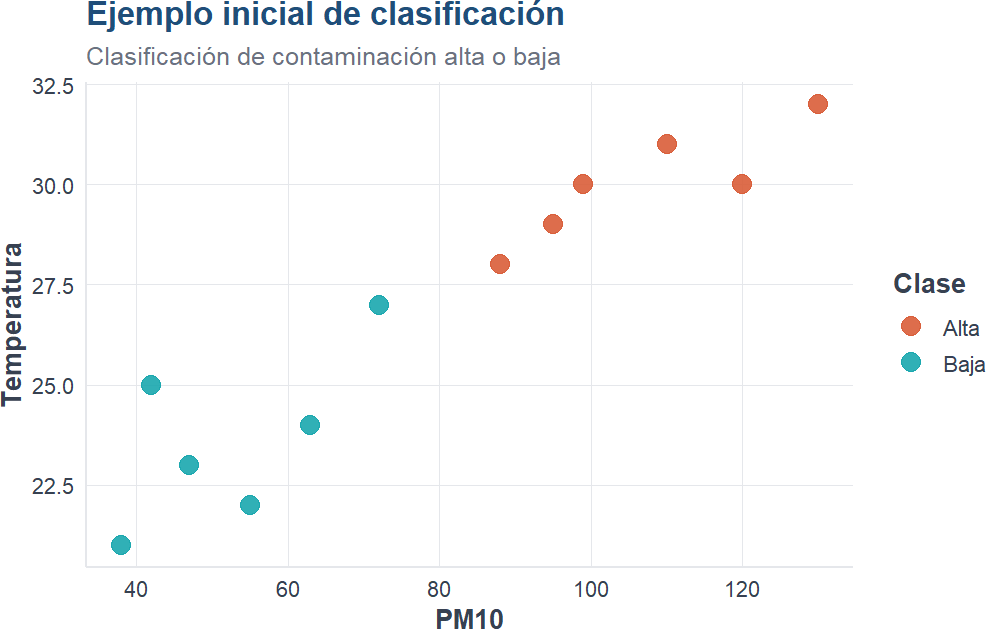
\includegraphics[width=0.92\linewidth,height=\textheight,keepaspectratio]{01-introduccion_files/figure-pdf/grafica-introduccion-1.png}

\begin{tcolorbox}[enhanced jigsaw, arc=.35mm, bottomrule=.15mm, bottomtitle=1mm, breakable, colback=white, colbacktitle=quarto-callout-note-color!10!white, colframe=quarto-callout-note-color-frame, coltitle=black, left=2mm, leftrule=.75mm, opacityback=0, opacitybacktitle=0.6, rightrule=.15mm, title=\textcolor{quarto-callout-note-color}{\faInfo}\hspace{0.5em}{Explicación del código}, titlerule=0mm, toprule=.15mm, toptitle=1mm]

La gráfica coloca PM10 en el eje horizontal, temperatura en el eje
vertical y usa color para distinguir la clase.

\end{tcolorbox}

\begin{tcolorbox}[enhanced jigsaw, arc=.35mm, bottomrule=.15mm, bottomtitle=1mm, breakable, colback=white, colbacktitle=quarto-callout-tip-color!10!white, colframe=quarto-callout-tip-color-frame, coltitle=black, left=2mm, leftrule=.75mm, opacityback=0, opacitybacktitle=0.6, rightrule=.15mm, title=\textcolor{quarto-callout-tip-color}{\faLightbulb}\hspace{0.5em}{Interpretación del resultado}, titlerule=0mm, toprule=.15mm, toptitle=1mm]

Los puntos permiten visualizar si las clases se separan. Esta es la idea
básica detrás de muchos métodos de clasificación.

\end{tcolorbox}

\section{División entre entrenamiento y
prueba}\label{divisiuxf3n-entre-entrenamiento-y-prueba}

\begin{Shaded}
\begin{Highlighting}[]
\FunctionTok{set.seed}\NormalTok{(}\DecValTok{123}\NormalTok{)}
\NormalTok{n }\OtherTok{\textless{}{-}} \FunctionTok{nrow}\NormalTok{(datos)}
\NormalTok{indices\_entrenamiento }\OtherTok{\textless{}{-}} \FunctionTok{sample}\NormalTok{(}\DecValTok{1}\SpecialCharTok{:}\NormalTok{n, }\AttributeTok{size =} \FunctionTok{round}\NormalTok{(}\FloatTok{0.7} \SpecialCharTok{*}\NormalTok{ n))}

\NormalTok{entrenamiento }\OtherTok{\textless{}{-}}\NormalTok{ datos[indices\_entrenamiento, ]}
\NormalTok{prueba }\OtherTok{\textless{}{-}}\NormalTok{ datos[}\SpecialCharTok{{-}}\NormalTok{indices\_entrenamiento, ]}

\NormalTok{entrenamiento}
\end{Highlighting}
\end{Shaded}

\begin{verbatim}
   dia pm10 temperatura humedad clase
3    3   55          22      60  Baja
12  12   99          30      34  Alta
10  10  130          32      28  Alta
2    2   88          28      35  Alta
6    6   95          29      33  Alta
11  11   47          23      62  Baja
5    5   63          24      55  Baja
4    4  120          30      30  Alta
\end{verbatim}

\begin{Shaded}
\begin{Highlighting}[]
\NormalTok{prueba}
\end{Highlighting}
\end{Shaded}

\begin{verbatim}
  dia pm10 temperatura humedad clase
1   1   42          25      40  Baja
7   7   38          21      65  Baja
8   8  110          31      29  Alta
9   9   72          27      42  Baja
\end{verbatim}

\begin{tcolorbox}[enhanced jigsaw, arc=.35mm, bottomrule=.15mm, bottomtitle=1mm, breakable, colback=white, colbacktitle=quarto-callout-note-color!10!white, colframe=quarto-callout-note-color-frame, coltitle=black, left=2mm, leftrule=.75mm, opacityback=0, opacitybacktitle=0.6, rightrule=.15mm, title=\textcolor{quarto-callout-note-color}{\faInfo}\hspace{0.5em}{Explicación del código}, titlerule=0mm, toprule=.15mm, toptitle=1mm]

Se divide la base en dos partes: una para entrenar el modelo y otra para
evaluar cómo funciona con datos no usados durante el ajuste.

\end{tcolorbox}

\section{Primer clasificador basado en una
regla}\label{primer-clasificador-basado-en-una-regla}

\begin{Shaded}
\begin{Highlighting}[]
\NormalTok{datos}\SpecialCharTok{$}\NormalTok{prediccion\_regla }\OtherTok{\textless{}{-}} \FunctionTok{ifelse}\NormalTok{(datos}\SpecialCharTok{$}\NormalTok{pm10 }\SpecialCharTok{\textgreater{}} \DecValTok{75}\NormalTok{, }\StringTok{"Alta"}\NormalTok{, }\StringTok{"Baja"}\NormalTok{)}

\NormalTok{tabla\_confusion }\OtherTok{\textless{}{-}} \FunctionTok{table}\NormalTok{(}
  \AttributeTok{Real =}\NormalTok{ datos}\SpecialCharTok{$}\NormalTok{clase,}
  \AttributeTok{Predicho =}\NormalTok{ datos}\SpecialCharTok{$}\NormalTok{prediccion\_regla}
\NormalTok{)}

\NormalTok{tabla\_confusion}
\end{Highlighting}
\end{Shaded}

\begin{verbatim}
      Predicho
Real   Alta Baja
  Alta    6    0
  Baja    0    6
\end{verbatim}

\begin{Shaded}
\begin{Highlighting}[]
\FunctionTok{mean}\NormalTok{(datos}\SpecialCharTok{$}\NormalTok{clase }\SpecialCharTok{==}\NormalTok{ datos}\SpecialCharTok{$}\NormalTok{prediccion\_regla)}
\end{Highlighting}
\end{Shaded}

\begin{verbatim}
[1] 1
\end{verbatim}

\begin{tcolorbox}[enhanced jigsaw, arc=.35mm, bottomrule=.15mm, bottomtitle=1mm, breakable, colback=white, colbacktitle=quarto-callout-tip-color!10!white, colframe=quarto-callout-tip-color-frame, coltitle=black, left=2mm, leftrule=.75mm, opacityback=0, opacitybacktitle=0.6, rightrule=.15mm, title=\textcolor{quarto-callout-tip-color}{\faLightbulb}\hspace{0.5em}{Interpretación del resultado}, titlerule=0mm, toprule=.15mm, toptitle=1mm]

La matriz de confusión compara la clase real contra la clase predicha.
La exactitud mide la proporción de aciertos.

\end{tcolorbox}

\section{Conclusión}\label{conclusiuxf3n}

El aprendizaje automático permite construir modelos que aprenden
patrones a partir de datos. En este capítulo vimos la diferencia entre
reglas manuales y aprendizaje a partir de ejemplos.

\bookmarksetup{startatroot}

\chapter{Preparación de datos
reales}\label{preparaciuxf3n-de-datos-reales}

\section{Objetivos del capítulo}\label{objetivos-del-capuxedtulo-1}

Al finalizar este capítulo, el lector será capaz de leer una base real,
seleccionar variables, construir una variable respuesta y guardar una
base preparada para modelado.

\section{Introducción}\label{introducciuxf3n-1}

En la práctica profesional, los datos reales casi nunca vienen
preparados. Antes de aplicar un algoritmo necesitamos revisar, limpiar,
transformar y documentar los datos.

\section{Cargar paquetes}\label{cargar-paquetes}

\begin{Shaded}
\begin{Highlighting}[]
\FunctionTok{library}\NormalTok{(readr)}
\FunctionTok{library}\NormalTok{(dplyr)}
\FunctionTok{library}\NormalTok{(ggplot2)}
\FunctionTok{library}\NormalTok{(stringr)}
\FunctionTok{source}\NormalTok{(}\StringTok{"util\_graficas.R"}\NormalTok{)}
\end{Highlighting}
\end{Shaded}

\begin{tcolorbox}[enhanced jigsaw, arc=.35mm, bottomrule=.15mm, bottomtitle=1mm, breakable, colback=white, colbacktitle=quarto-callout-note-color!10!white, colframe=quarto-callout-note-color-frame, coltitle=black, left=2mm, leftrule=.75mm, opacityback=0, opacitybacktitle=0.6, rightrule=.15mm, title=\textcolor{quarto-callout-note-color}{\faInfo}\hspace{0.5em}{Explicación del código}, titlerule=0mm, toprule=.15mm, toptitle=1mm]

Se cargan paquetes para leer archivos CSV, transformar datos, trabajar
con texto y crear gráficas profesionales.

\end{tcolorbox}

\section{Leer el archivo CSV}\label{leer-el-archivo-csv}

\begin{Shaded}
\begin{Highlighting}[]
\NormalTok{ruta\_atus }\OtherTok{\textless{}{-}} \StringTok{"datos/atus\_2024.csv"}
\FunctionTok{file.exists}\NormalTok{(ruta\_atus)}
\end{Highlighting}
\end{Shaded}

\begin{verbatim}
[1] TRUE
\end{verbatim}

\begin{Shaded}
\begin{Highlighting}[]
\ControlFlowTok{if}\NormalTok{ (}\FunctionTok{file.exists}\NormalTok{(ruta\_atus)) \{}
\NormalTok{  atus }\OtherTok{\textless{}{-}} \FunctionTok{read\_csv}\NormalTok{(}\AttributeTok{file =}\NormalTok{ ruta\_atus, }\AttributeTok{show\_col\_types =} \ConstantTok{FALSE}\NormalTok{, }\AttributeTok{locale =} \FunctionTok{locale}\NormalTok{(}\AttributeTok{encoding =} \StringTok{"UTF{-}8"}\NormalTok{))}
  \FunctionTok{print}\NormalTok{(}\StringTok{"Archivo leído correctamente."}\NormalTok{)}
\NormalTok{\} }\ControlFlowTok{else}\NormalTok{ \{}
\NormalTok{  atus }\OtherTok{\textless{}{-}} \ConstantTok{NULL}
  \FunctionTok{print}\NormalTok{(}\StringTok{"El archivo atus\_2024.csv todavía no está disponible en la carpeta datos."}\NormalTok{)}
\NormalTok{\}}
\end{Highlighting}
\end{Shaded}

\begin{verbatim}
[1] "Archivo leído correctamente."
\end{verbatim}

\begin{tcolorbox}[enhanced jigsaw, arc=.35mm, bottomrule=.15mm, bottomtitle=1mm, breakable, colback=white, colbacktitle=quarto-callout-tip-color!10!white, colframe=quarto-callout-tip-color-frame, coltitle=black, left=2mm, leftrule=.75mm, opacityback=0, opacitybacktitle=0.6, rightrule=.15mm, title=\textcolor{quarto-callout-tip-color}{\faLightbulb}\hspace{0.5em}{Interpretación del resultado}, titlerule=0mm, toprule=.15mm, toptitle=1mm]

Si aparece \texttt{TRUE} y el mensaje de lectura correcta, el archivo
está disponible y se puede continuar con la preparación.

\end{tcolorbox}

\section{Primer vistazo a los datos}\label{primer-vistazo-a-los-datos}

\begin{Shaded}
\begin{Highlighting}[]
\ControlFlowTok{if}\NormalTok{ (}\SpecialCharTok{!}\FunctionTok{is.null}\NormalTok{(atus)) \{}
  \FunctionTok{data.frame}\NormalTok{(}\AttributeTok{filas =} \FunctionTok{nrow}\NormalTok{(atus), }\AttributeTok{columnas =} \FunctionTok{ncol}\NormalTok{(atus))}
  \FunctionTok{head}\NormalTok{(atus)}
\NormalTok{\}}
\end{Highlighting}
\end{Shaded}

\begin{verbatim}
# A tibble: 6 x 45
  COBERTURA ID_ENTIDAD ID_MUNICIPIO  ANIO MES   ID_HORA ID_MINUTO ID_DIA
  <chr>     <chr>      <chr>        <dbl> <chr> <chr>   <chr>     <chr> 
1 Municipal 01         001           2024 01    02      25        01    
2 Municipal 01         001           2024 01    03      40        01    
3 Municipal 01         001           2024 01    04      37        01    
4 Municipal 01         001           2024 01    05      00        01    
5 Municipal 01         001           2024 01    06      45        01    
6 Municipal 01         001           2024 01    07      30        01    
# i 37 more variables: DIASEMANA <chr>, URBANA <chr>, SUBURBANA <chr>,
#   TIPACCID <chr>, AUTOMOVIL <dbl>, CAMPASAJ <dbl>, MICROBUS <dbl>,
#   PASCAMION <dbl>, OMNIBUS <dbl>, TRANVIA <dbl>, CAMIONETA <dbl>,
#   CAMION <dbl>, TRACTOR <dbl>, FERROCARRI <dbl>, MOTOCICLET <dbl>,
#   BICICLETA <dbl>, OTROVEHIC <dbl>, CAUSAACCI <chr>, CAPAROD <chr>,
#   SEXO <chr>, ALIENTO <chr>, CINTURON <chr>, ID_EDAD <dbl>, CONDMUERTO <dbl>,
#   CONDHERIDO <dbl>, PASAMUERTO <dbl>, PASAHERIDO <dbl>, PEATMUERTO <dbl>, ...
\end{verbatim}

\begin{tcolorbox}[enhanced jigsaw, arc=.35mm, bottomrule=.15mm, bottomtitle=1mm, breakable, colback=white, colbacktitle=quarto-callout-note-color!10!white, colframe=quarto-callout-note-color-frame, coltitle=black, left=2mm, leftrule=.75mm, opacityback=0, opacitybacktitle=0.6, rightrule=.15mm, title=\textcolor{quarto-callout-note-color}{\faInfo}\hspace{0.5em}{Explicación del código}, titlerule=0mm, toprule=.15mm, toptitle=1mm]

Se revisan las dimensiones de la base y las primeras filas para
confirmar que las variables esperadas están presentes.

\end{tcolorbox}

\section{Variables de interés}\label{variables-de-interuxe9s}

\begin{Shaded}
\begin{Highlighting}[]
\NormalTok{variables\_interes }\OtherTok{\textless{}{-}} \FunctionTok{c}\NormalTok{(}
  \StringTok{"ANIO"}\NormalTok{, }\StringTok{"MES"}\NormalTok{, }\StringTok{"ID\_ENTIDAD"}\NormalTok{, }\StringTok{"ID\_MUNICIPIO"}\NormalTok{, }\StringTok{"ID\_HORA"}\NormalTok{, }\StringTok{"ID\_DIA"}\NormalTok{,}
  \StringTok{"DIASEMANA"}\NormalTok{, }\StringTok{"TIPACCID"}\NormalTok{, }\StringTok{"CAUSAACCI"}\NormalTok{, }\StringTok{"CLASACC"}
\NormalTok{)}

\ControlFlowTok{if}\NormalTok{ (}\SpecialCharTok{!}\FunctionTok{is.null}\NormalTok{(atus)) \{}
  \FunctionTok{names}\NormalTok{(atus) }\OtherTok{\textless{}{-}} \FunctionTok{toupper}\NormalTok{(}\FunctionTok{names}\NormalTok{(atus))}
\NormalTok{  variables\_existentes }\OtherTok{\textless{}{-}} \FunctionTok{intersect}\NormalTok{(variables\_interes, }\FunctionTok{names}\NormalTok{(atus))}
\NormalTok{  atus\_base }\OtherTok{\textless{}{-}}\NormalTok{ atus }\SpecialCharTok{|\textgreater{}} \FunctionTok{select}\NormalTok{(}\FunctionTok{all\_of}\NormalTok{(variables\_existentes))}
  \FunctionTok{head}\NormalTok{(atus\_base)}
\NormalTok{\}}
\end{Highlighting}
\end{Shaded}

\begin{verbatim}
# A tibble: 6 x 10
   ANIO MES   ID_ENTIDAD ID_MUNICIPIO ID_HORA ID_DIA DIASEMANA TIPACCID         
  <dbl> <chr> <chr>      <chr>        <chr>   <chr>  <chr>     <chr>            
1  2024 01    01         001          02      01     lunes     Colisión con veh~
2  2024 01    01         001          03      01     lunes     Colisión con obj~
3  2024 01    01         001          04      01     lunes     Colisión con pea~
4  2024 01    01         001          05      01     lunes     Colisión con obj~
5  2024 01    01         001          06      01     lunes     Colisión con obj~
6  2024 01    01         001          07      01     lunes     Colisión con veh~
# i 2 more variables: CAUSAACCI <chr>, CLASACC <chr>
\end{verbatim}

\begin{tcolorbox}[enhanced jigsaw, arc=.35mm, bottomrule=.15mm, bottomtitle=1mm, breakable, colback=white, colbacktitle=quarto-callout-tip-color!10!white, colframe=quarto-callout-tip-color-frame, coltitle=black, left=2mm, leftrule=.75mm, opacityback=0, opacitybacktitle=0.6, rightrule=.15mm, title=\textcolor{quarto-callout-tip-color}{\faLightbulb}\hspace{0.5em}{Interpretación del resultado}, titlerule=0mm, toprule=.15mm, toptitle=1mm]

La base queda reducida a variables útiles para el primer problema de
clasificación.

\end{tcolorbox}

\section{Crear variable respuesta}\label{crear-variable-respuesta}

\begin{Shaded}
\begin{Highlighting}[]
\ControlFlowTok{if}\NormalTok{ (}\FunctionTok{exists}\NormalTok{(}\StringTok{"atus\_base"}\NormalTok{) }\SpecialCharTok{\&\&} \StringTok{"CLASACC"} \SpecialCharTok{\%in\%} \FunctionTok{names}\NormalTok{(atus\_base)) \{}
\NormalTok{  atus\_modelo }\OtherTok{\textless{}{-}}\NormalTok{ atus\_base }\SpecialCharTok{|\textgreater{}}
    \FunctionTok{mutate}\NormalTok{(}
      \AttributeTok{CLASACC\_TXT =} \FunctionTok{str\_to\_lower}\NormalTok{(}\FunctionTok{as.character}\NormalTok{(CLASACC)),}
      \AttributeTok{accidente\_con\_victimas =} \FunctionTok{case\_when}\NormalTok{(}
        \FunctionTok{str\_detect}\NormalTok{(CLASACC\_TXT, }\StringTok{"sólo daños"}\NormalTok{) }\SpecialCharTok{\textasciitilde{}} \StringTok{"Solo daños"}\NormalTok{,}
        \FunctionTok{str\_detect}\NormalTok{(CLASACC\_TXT, }\StringTok{"solo daños"}\NormalTok{) }\SpecialCharTok{\textasciitilde{}} \StringTok{"Solo daños"}\NormalTok{,}
        \FunctionTok{str\_detect}\NormalTok{(CLASACC\_TXT, }\StringTok{"daños"}\NormalTok{) }\SpecialCharTok{\textasciitilde{}} \StringTok{"Solo daños"}\NormalTok{,}
        \FunctionTok{str\_detect}\NormalTok{(CLASACC\_TXT, }\StringTok{"no fatal"}\NormalTok{) }\SpecialCharTok{\textasciitilde{}} \StringTok{"Con víctimas"}\NormalTok{,}
        \FunctionTok{str\_detect}\NormalTok{(CLASACC\_TXT, }\StringTok{"fatal"}\NormalTok{) }\SpecialCharTok{\textasciitilde{}} \StringTok{"Con víctimas"}\NormalTok{,}
        \ConstantTok{TRUE} \SpecialCharTok{\textasciitilde{}} \ConstantTok{NA\_character\_}
\NormalTok{      )}
\NormalTok{    ) }\SpecialCharTok{|\textgreater{}}
    \FunctionTok{filter}\NormalTok{(}\SpecialCharTok{!}\FunctionTok{is.na}\NormalTok{(accidente\_con\_victimas))}

  \FunctionTok{table}\NormalTok{(atus\_modelo}\SpecialCharTok{$}\NormalTok{accidente\_con\_victimas)}
\NormalTok{\}}
\end{Highlighting}
\end{Shaded}

\begin{verbatim}

Con víctimas   Solo daños 
       68108       322519 
\end{verbatim}

\begin{tcolorbox}[enhanced jigsaw, arc=.35mm, bottomrule=.15mm, bottomtitle=1mm, breakable, colback=white, colbacktitle=quarto-callout-note-color!10!white, colframe=quarto-callout-note-color-frame, coltitle=black, left=2mm, leftrule=.75mm, opacityback=0, opacitybacktitle=0.6, rightrule=.15mm, title=\textcolor{quarto-callout-note-color}{\faInfo}\hspace{0.5em}{Explicación del código}, titlerule=0mm, toprule=.15mm, toptitle=1mm]

La variable \texttt{CLASACC} se transforma en una respuesta binaria:
accidentes con víctimas y accidentes de solo daños.

\end{tcolorbox}

\section{Preparar variables finales}\label{preparar-variables-finales}

\begin{Shaded}
\begin{Highlighting}[]
\ControlFlowTok{if}\NormalTok{ (}\FunctionTok{exists}\NormalTok{(}\StringTok{"atus\_modelo"}\NormalTok{)) \{}
\NormalTok{  atus\_ml }\OtherTok{\textless{}{-}}\NormalTok{ atus\_modelo }\SpecialCharTok{|\textgreater{}}
    \FunctionTok{mutate}\NormalTok{(}
      \AttributeTok{MES =} \FunctionTok{as.factor}\NormalTok{(MES),}
      \AttributeTok{ID\_HORA =} \FunctionTok{as.character}\NormalTok{(ID\_HORA),}
      \AttributeTok{DIASEMANA =} \FunctionTok{as.factor}\NormalTok{(DIASEMANA),}
      \AttributeTok{TIPACCID =} \FunctionTok{as.factor}\NormalTok{(TIPACCID),}
      \AttributeTok{CAUSAACCI =} \FunctionTok{as.factor}\NormalTok{(CAUSAACCI),}
      \AttributeTok{accidente\_con\_victimas =} \FunctionTok{factor}\NormalTok{(accidente\_con\_victimas, }\AttributeTok{levels =} \FunctionTok{c}\NormalTok{(}\StringTok{"Con víctimas"}\NormalTok{, }\StringTok{"Solo daños"}\NormalTok{))}
\NormalTok{    ) }\SpecialCharTok{|\textgreater{}}
    \FunctionTok{select}\NormalTok{(accidente\_con\_victimas, MES, ID\_HORA, DIASEMANA, TIPACCID, CAUSAACCI) }\SpecialCharTok{|\textgreater{}}
    \FunctionTok{na.omit}\NormalTok{()}

  \FunctionTok{data.frame}\NormalTok{(}\AttributeTok{filas =} \FunctionTok{nrow}\NormalTok{(atus\_ml), }\AttributeTok{columnas =} \FunctionTok{ncol}\NormalTok{(atus\_ml))}
\NormalTok{\}}
\end{Highlighting}
\end{Shaded}

\begin{verbatim}
   filas columnas
1 390627        6
\end{verbatim}

\begin{tcolorbox}[enhanced jigsaw, arc=.35mm, bottomrule=.15mm, bottomtitle=1mm, breakable, colback=white, colbacktitle=quarto-callout-tip-color!10!white, colframe=quarto-callout-tip-color-frame, coltitle=black, left=2mm, leftrule=.75mm, opacityback=0, opacitybacktitle=0.6, rightrule=.15mm, title=\textcolor{quarto-callout-tip-color}{\faLightbulb}\hspace{0.5em}{Interpretación del resultado}, titlerule=0mm, toprule=.15mm, toptitle=1mm]

La base final queda lista para análisis exploratorio y modelado. Cada
fila representa un accidente y cada columna una variable útil.

\end{tcolorbox}

\section{Guardar base preparada}\label{guardar-base-preparada}

\begin{Shaded}
\begin{Highlighting}[]
\ControlFlowTok{if}\NormalTok{ (}\FunctionTok{exists}\NormalTok{(}\StringTok{"atus\_ml"}\NormalTok{)) \{}
  \ControlFlowTok{if}\NormalTok{ (}\SpecialCharTok{!}\FunctionTok{dir.exists}\NormalTok{(}\StringTok{"datos"}\NormalTok{)) }\FunctionTok{dir.create}\NormalTok{(}\StringTok{"datos"}\NormalTok{)}
  \FunctionTok{write\_csv}\NormalTok{(atus\_ml, }\StringTok{"datos/atus\_ml\_preparado.csv"}\NormalTok{)}
\NormalTok{\}}
\end{Highlighting}
\end{Shaded}

\begin{tcolorbox}[enhanced jigsaw, arc=.35mm, bottomrule=.15mm, bottomtitle=1mm, breakable, colback=white, colbacktitle=quarto-callout-note-color!10!white, colframe=quarto-callout-note-color-frame, coltitle=black, left=2mm, leftrule=.75mm, opacityback=0, opacitybacktitle=0.6, rightrule=.15mm, title=\textcolor{quarto-callout-note-color}{\faInfo}\hspace{0.5em}{Explicación del código}, titlerule=0mm, toprule=.15mm, toptitle=1mm]

La base preparada se guarda para no repetir todo el proceso de limpieza
en los capítulos siguientes.

\end{tcolorbox}

\section{Resumen del capítulo}\label{resumen-del-capuxedtulo}

En este capítulo leímos una base real, seleccionamos variables,
construimos una variable respuesta y guardamos una base preparada para
aprendizaje automático.

\bookmarksetup{startatroot}

\chapter{Análisis exploratorio de
datos}\label{anuxe1lisis-exploratorio-de-datos}

\section{Objetivos del capítulo}\label{objetivos-del-capuxedtulo-2}

Al finalizar este capítulo, el lector será capaz de cargar una base
preparada, revisar su estructura, calcular frecuencias, construir
gráficas e interpretar patrones iniciales.

\section{Cargar paquetes y base}\label{cargar-paquetes-y-base}

\begin{Shaded}
\begin{Highlighting}[]
\FunctionTok{library}\NormalTok{(readr)}
\FunctionTok{library}\NormalTok{(dplyr)}
\FunctionTok{library}\NormalTok{(ggplot2)}
\FunctionTok{source}\NormalTok{(}\StringTok{"util\_graficas.R"}\NormalTok{)}

\NormalTok{ruta\_atus\_ml }\OtherTok{\textless{}{-}} \StringTok{"datos/atus\_ml\_preparado.csv"}

\ControlFlowTok{if}\NormalTok{ (}\FunctionTok{file.exists}\NormalTok{(ruta\_atus\_ml)) \{}
\NormalTok{  atus\_ml }\OtherTok{\textless{}{-}} \FunctionTok{read\_csv}\NormalTok{(ruta\_atus\_ml, }\AttributeTok{show\_col\_types =} \ConstantTok{FALSE}\NormalTok{)}
  \FunctionTok{print}\NormalTok{(}\StringTok{"Base preparada cargada correctamente."}\NormalTok{)}
\NormalTok{\} }\ControlFlowTok{else}\NormalTok{ \{}
\NormalTok{  atus\_ml }\OtherTok{\textless{}{-}} \ConstantTok{NULL}
  \FunctionTok{print}\NormalTok{(}\StringTok{"No se encontró el archivo datos/atus\_ml\_preparado.csv. Ejecuta primero el capítulo 2."}\NormalTok{)}
\NormalTok{\}}
\end{Highlighting}
\end{Shaded}

\begin{verbatim}
[1] "Base preparada cargada correctamente."
\end{verbatim}

\begin{tcolorbox}[enhanced jigsaw, arc=.35mm, bottomrule=.15mm, bottomtitle=1mm, breakable, colback=white, colbacktitle=quarto-callout-note-color!10!white, colframe=quarto-callout-note-color-frame, coltitle=black, left=2mm, leftrule=.75mm, opacityback=0, opacitybacktitle=0.6, rightrule=.15mm, title=\textcolor{quarto-callout-note-color}{\faInfo}\hspace{0.5em}{Explicación del código}, titlerule=0mm, toprule=.15mm, toptitle=1mm]

Se carga la base preparada en el capítulo anterior. Esto permite empezar
directamente con el análisis exploratorio.

\end{tcolorbox}

\section{Preparar variables}\label{preparar-variables}

\begin{Shaded}
\begin{Highlighting}[]
\ControlFlowTok{if}\NormalTok{ (}\SpecialCharTok{!}\FunctionTok{is.null}\NormalTok{(atus\_ml)) \{}
\NormalTok{  atus\_ml }\OtherTok{\textless{}{-}}\NormalTok{ atus\_ml }\SpecialCharTok{|\textgreater{}}
    \FunctionTok{mutate}\NormalTok{(}
      \AttributeTok{ID\_HORA\_NUM =} \FunctionTok{as.numeric}\NormalTok{(ID\_HORA),}
      \AttributeTok{MES\_NUM =} \FunctionTok{as.numeric}\NormalTok{(MES),}
      \AttributeTok{MES\_FACTOR =} \FunctionTok{factor}\NormalTok{(}\FunctionTok{sprintf}\NormalTok{(}\StringTok{"\%02d"}\NormalTok{, MES\_NUM), }\AttributeTok{levels =} \FunctionTok{sprintf}\NormalTok{(}\StringTok{"\%02d"}\NormalTok{, }\DecValTok{1}\SpecialCharTok{:}\DecValTok{12}\NormalTok{)),}
      \AttributeTok{accidente\_con\_victimas =} \FunctionTok{factor}\NormalTok{(accidente\_con\_victimas, }\AttributeTok{levels =} \FunctionTok{c}\NormalTok{(}\StringTok{"Con víctimas"}\NormalTok{, }\StringTok{"Solo daños"}\NormalTok{))}
\NormalTok{    )}
\NormalTok{\}}
\end{Highlighting}
\end{Shaded}

\begin{tcolorbox}[enhanced jigsaw, arc=.35mm, bottomrule=.15mm, bottomtitle=1mm, breakable, colback=white, colbacktitle=quarto-callout-note-color!10!white, colframe=quarto-callout-note-color-frame, coltitle=black, left=2mm, leftrule=.75mm, opacityback=0, opacitybacktitle=0.6, rightrule=.15mm, title=\textcolor{quarto-callout-note-color}{\faInfo}\hspace{0.5em}{Explicación del código}, titlerule=0mm, toprule=.15mm, toptitle=1mm]

Se crean variables numéricas y factores ordenados para facilitar tablas
y gráficas.

\end{tcolorbox}

\section{Distribución de la variable
respuesta}\label{distribuciuxf3n-de-la-variable-respuesta}

\begin{Shaded}
\begin{Highlighting}[]
\ControlFlowTok{if}\NormalTok{ (}\SpecialCharTok{!}\FunctionTok{is.null}\NormalTok{(atus\_ml)) \{}
\NormalTok{  tabla\_clase }\OtherTok{\textless{}{-}} \FunctionTok{table}\NormalTok{(atus\_ml}\SpecialCharTok{$}\NormalTok{accidente\_con\_victimas)}
  \FunctionTok{round}\NormalTok{(}\DecValTok{100} \SpecialCharTok{*} \FunctionTok{prop.table}\NormalTok{(tabla\_clase), }\DecValTok{2}\NormalTok{)}
\NormalTok{\}}
\end{Highlighting}
\end{Shaded}

\begin{verbatim}

Con víctimas   Solo daños 
       17.44        82.56 
\end{verbatim}

\begin{Shaded}
\begin{Highlighting}[]
\ControlFlowTok{if}\NormalTok{ (}\SpecialCharTok{!}\FunctionTok{is.null}\NormalTok{(atus\_ml)) \{}
  \FunctionTok{ggplot}\NormalTok{(atus\_ml, }\FunctionTok{aes}\NormalTok{(}\AttributeTok{x =}\NormalTok{ accidente\_con\_victimas, }\AttributeTok{fill =}\NormalTok{ accidente\_con\_victimas)) }\SpecialCharTok{+}
    \FunctionTok{geom\_bar}\NormalTok{(}\AttributeTok{width =} \FloatTok{0.7}\NormalTok{) }\SpecialCharTok{+}
    \FunctionTok{escala\_clases\_fill}\NormalTok{() }\SpecialCharTok{+}
    \FunctionTok{scale\_y\_continuous}\NormalTok{(}\AttributeTok{labels =}\NormalTok{ etiqueta\_numero) }\SpecialCharTok{+}
    \FunctionTok{labs}\NormalTok{(}
      \AttributeTok{title =} \StringTok{"Distribución de accidentes según presencia de víctimas"}\NormalTok{,}
      \AttributeTok{subtitle =} \StringTok{"Comparación entre clases"}\NormalTok{,}
      \AttributeTok{x =} \StringTok{"Clase"}\NormalTok{,}
      \AttributeTok{y =} \StringTok{"Número de accidentes"}\NormalTok{,}
      \AttributeTok{fill =} \StringTok{"Clase"}
\NormalTok{    ) }\SpecialCharTok{+}
    \FunctionTok{tema\_libro}\NormalTok{() }\SpecialCharTok{+}
    \FunctionTok{theme}\NormalTok{(}\AttributeTok{legend.position =} \StringTok{"none"}\NormalTok{)}
\NormalTok{\}}
\end{Highlighting}
\end{Shaded}

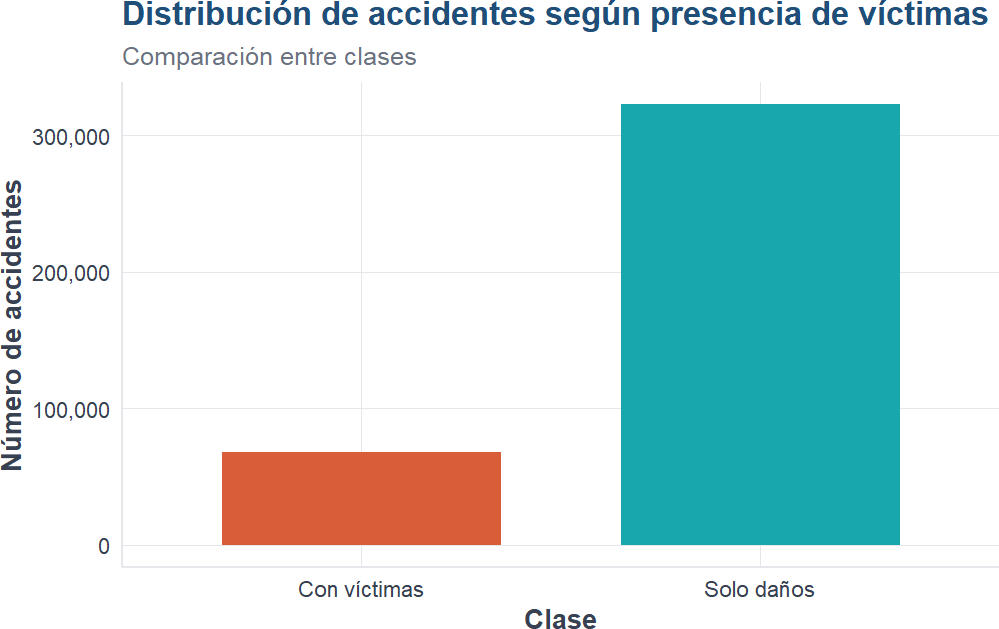
\includegraphics[width=0.92\linewidth,height=\textheight,keepaspectratio]{03-analisis-exploratorio_files/figure-pdf/distribucion-respuesta-1.png}

\begin{tcolorbox}[enhanced jigsaw, arc=.35mm, bottomrule=.15mm, bottomtitle=1mm, breakable, colback=white, colbacktitle=quarto-callout-tip-color!10!white, colframe=quarto-callout-tip-color-frame, coltitle=black, left=2mm, leftrule=.75mm, opacityback=0, opacitybacktitle=0.6, rightrule=.15mm, title=\textcolor{quarto-callout-tip-color}{\faLightbulb}\hspace{0.5em}{Interpretación del resultado}, titlerule=0mm, toprule=.15mm, toptitle=1mm]

La base está desbalanceada: hay más accidentes de solo daños que
accidentes con víctimas. Esto será importante al evaluar modelos.

\end{tcolorbox}

\section{Accidentes por mes}\label{accidentes-por-mes}

\begin{Shaded}
\begin{Highlighting}[]
\ControlFlowTok{if}\NormalTok{ (}\SpecialCharTok{!}\FunctionTok{is.null}\NormalTok{(atus\_ml)) \{}
\NormalTok{  accidentes\_mes }\OtherTok{\textless{}{-}}\NormalTok{ atus\_ml }\SpecialCharTok{|\textgreater{}} \FunctionTok{count}\NormalTok{(MES\_FACTOR, }\AttributeTok{name =} \StringTok{"n"}\NormalTok{) }\SpecialCharTok{|\textgreater{}} \FunctionTok{arrange}\NormalTok{(MES\_FACTOR)}
\NormalTok{  accidentes\_mes}
\NormalTok{\}}
\end{Highlighting}
\end{Shaded}

\begin{verbatim}
# A tibble: 12 x 2
   MES_FACTOR     n
   <fct>      <int>
 1 01         31600
 2 02         32208
 3 03         33237
 4 04         32666
 5 05         34665
 6 06         31737
 7 07         30062
 8 08         31800
 9 09         31351
10 10         33771
11 11         34047
12 12         33483
\end{verbatim}

\begin{Shaded}
\begin{Highlighting}[]
\ControlFlowTok{if}\NormalTok{ (}\FunctionTok{exists}\NormalTok{(}\StringTok{"accidentes\_mes"}\NormalTok{)) \{}
  \FunctionTok{ggplot}\NormalTok{(accidentes\_mes, }\FunctionTok{aes}\NormalTok{(}\AttributeTok{x =}\NormalTok{ MES\_FACTOR, }\AttributeTok{y =}\NormalTok{ n)) }\SpecialCharTok{+}
    \FunctionTok{geom\_col}\NormalTok{(}\AttributeTok{fill =}\NormalTok{ col\_azul, }\AttributeTok{width =} \FloatTok{0.75}\NormalTok{) }\SpecialCharTok{+}
    \FunctionTok{scale\_y\_continuous}\NormalTok{(}\AttributeTok{labels =}\NormalTok{ etiqueta\_numero) }\SpecialCharTok{+}
    \FunctionTok{labs}\NormalTok{(}
      \AttributeTok{title =} \StringTok{"Número de accidentes por mes"}\NormalTok{,}
      \AttributeTok{subtitle =} \StringTok{"Base ATUS preparada"}\NormalTok{,}
      \AttributeTok{x =} \StringTok{"Mes"}\NormalTok{,}
      \AttributeTok{y =} \StringTok{"Número de accidentes"}
\NormalTok{    ) }\SpecialCharTok{+}
    \FunctionTok{tema\_libro}\NormalTok{()}
\NormalTok{\}}
\end{Highlighting}
\end{Shaded}

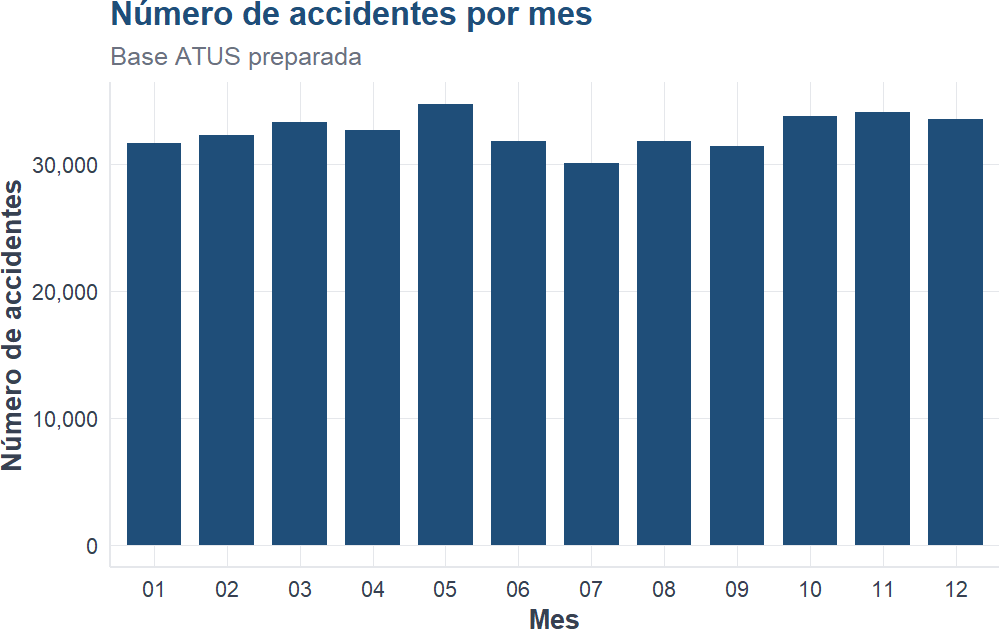
\includegraphics[width=0.92\linewidth,height=\textheight,keepaspectratio]{03-analisis-exploratorio_files/figure-pdf/accidentes-mes-1.png}

\begin{tcolorbox}[enhanced jigsaw, arc=.35mm, bottomrule=.15mm, bottomtitle=1mm, breakable, colback=white, colbacktitle=quarto-callout-note-color!10!white, colframe=quarto-callout-note-color-frame, coltitle=black, left=2mm, leftrule=.75mm, opacityback=0, opacitybacktitle=0.6, rightrule=.15mm, title=\textcolor{quarto-callout-note-color}{\faInfo}\hspace{0.5em}{Explicación del código}, titlerule=0mm, toprule=.15mm, toptitle=1mm]

Se cuentan los accidentes por mes y se visualizan con barras. El eje
vertical usa separadores de miles para facilitar la lectura.

\end{tcolorbox}

\section{Accidentes por hora del
día}\label{accidentes-por-hora-del-duxeda}

\begin{Shaded}
\begin{Highlighting}[]
\ControlFlowTok{if}\NormalTok{ (}\SpecialCharTok{!}\FunctionTok{is.null}\NormalTok{(atus\_ml)) \{}
\NormalTok{  accidentes\_hora }\OtherTok{\textless{}{-}}\NormalTok{ atus\_ml }\SpecialCharTok{|\textgreater{}} \FunctionTok{count}\NormalTok{(ID\_HORA\_NUM, }\AttributeTok{name =} \StringTok{"n"}\NormalTok{) }\SpecialCharTok{|\textgreater{}} \FunctionTok{arrange}\NormalTok{(ID\_HORA\_NUM)}

  \FunctionTok{ggplot}\NormalTok{(accidentes\_hora, }\FunctionTok{aes}\NormalTok{(}\AttributeTok{x =}\NormalTok{ ID\_HORA\_NUM, }\AttributeTok{y =}\NormalTok{ n)) }\SpecialCharTok{+}
    \FunctionTok{geom\_col}\NormalTok{(}\AttributeTok{fill =}\NormalTok{ col\_turquesa, }\AttributeTok{width =} \FloatTok{0.75}\NormalTok{) }\SpecialCharTok{+}
    \FunctionTok{scale\_x\_continuous}\NormalTok{(}\AttributeTok{breaks =} \DecValTok{0}\SpecialCharTok{:}\DecValTok{23}\NormalTok{) }\SpecialCharTok{+}
    \FunctionTok{scale\_y\_continuous}\NormalTok{(}\AttributeTok{labels =}\NormalTok{ etiqueta\_numero) }\SpecialCharTok{+}
    \FunctionTok{labs}\NormalTok{(}
      \AttributeTok{title =} \StringTok{"Número de accidentes por hora del día"}\NormalTok{,}
      \AttributeTok{x =} \StringTok{"Hora del día"}\NormalTok{,}
      \AttributeTok{y =} \StringTok{"Número de accidentes"}
\NormalTok{    ) }\SpecialCharTok{+}
    \FunctionTok{tema\_libro}\NormalTok{()}
\NormalTok{\}}
\end{Highlighting}
\end{Shaded}

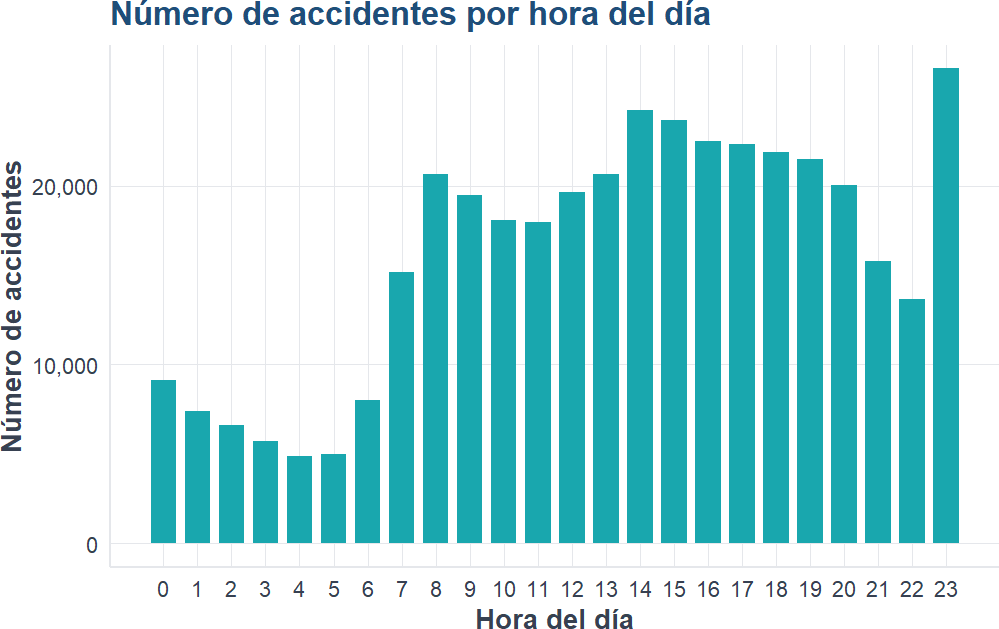
\includegraphics[width=0.92\linewidth,height=\textheight,keepaspectratio]{03-analisis-exploratorio_files/figure-pdf/accidentes-hora-1.png}

\begin{tcolorbox}[enhanced jigsaw, arc=.35mm, bottomrule=.15mm, bottomtitle=1mm, breakable, colback=white, colbacktitle=quarto-callout-tip-color!10!white, colframe=quarto-callout-tip-color-frame, coltitle=black, left=2mm, leftrule=.75mm, opacityback=0, opacitybacktitle=0.6, rightrule=.15mm, title=\textcolor{quarto-callout-tip-color}{\faLightbulb}\hspace{0.5em}{Interpretación del resultado}, titlerule=0mm, toprule=.15mm, toptitle=1mm]

La gráfica permite detectar horas con mayor concentración de accidentes.

\end{tcolorbox}

\section{Tipos de accidente más
frecuentes}\label{tipos-de-accidente-muxe1s-frecuentes}

\begin{Shaded}
\begin{Highlighting}[]
\ControlFlowTok{if}\NormalTok{ (}\SpecialCharTok{!}\FunctionTok{is.null}\NormalTok{(atus\_ml)) \{}
\NormalTok{  accidentes\_tipo\_top }\OtherTok{\textless{}{-}}\NormalTok{ atus\_ml }\SpecialCharTok{|\textgreater{}} \FunctionTok{count}\NormalTok{(TIPACCID, }\AttributeTok{name =} \StringTok{"n"}\NormalTok{) }\SpecialCharTok{|\textgreater{}} \FunctionTok{slice\_max}\NormalTok{(n, }\AttributeTok{n =} \DecValTok{10}\NormalTok{)}

  \FunctionTok{ggplot}\NormalTok{(accidentes\_tipo\_top, }\FunctionTok{aes}\NormalTok{(}\AttributeTok{x =} \FunctionTok{reorder}\NormalTok{(TIPACCID, n), }\AttributeTok{y =}\NormalTok{ n)) }\SpecialCharTok{+}
    \FunctionTok{geom\_col}\NormalTok{(}\AttributeTok{fill =}\NormalTok{ col\_azul, }\AttributeTok{width =} \FloatTok{0.75}\NormalTok{) }\SpecialCharTok{+}
    \FunctionTok{coord\_flip}\NormalTok{() }\SpecialCharTok{+}
    \FunctionTok{scale\_y\_continuous}\NormalTok{(}\AttributeTok{labels =}\NormalTok{ etiqueta\_numero) }\SpecialCharTok{+}
    \FunctionTok{labs}\NormalTok{(}
      \AttributeTok{title =} \StringTok{"Tipos de accidente más frecuentes"}\NormalTok{,}
      \AttributeTok{x =} \StringTok{"Tipo de accidente"}\NormalTok{,}
      \AttributeTok{y =} \StringTok{"Número de accidentes"}
\NormalTok{    ) }\SpecialCharTok{+}
    \FunctionTok{tema\_libro}\NormalTok{()}
\NormalTok{\}}
\end{Highlighting}
\end{Shaded}

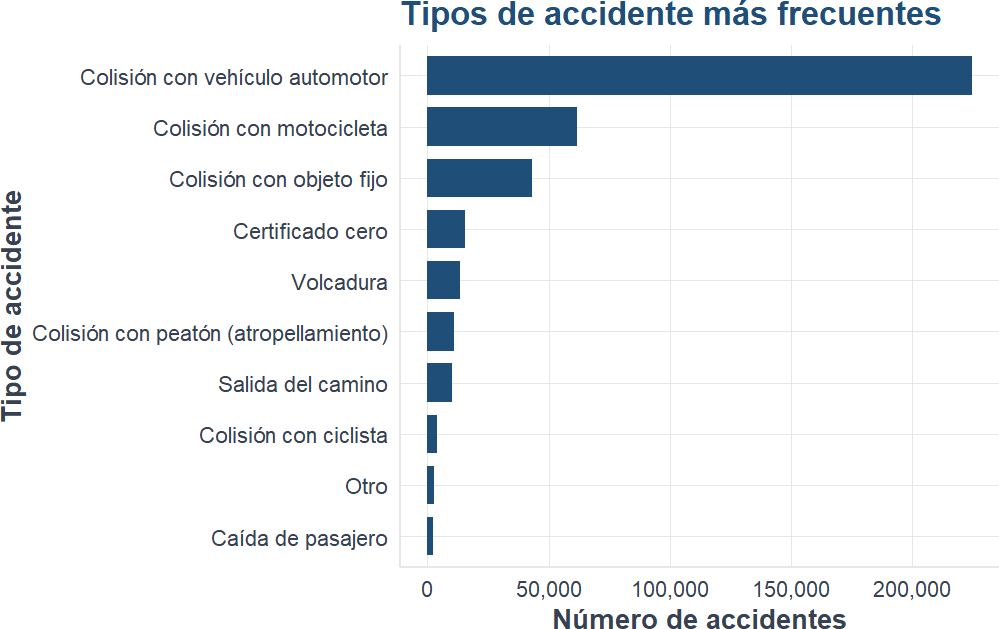
\includegraphics[width=0.92\linewidth,height=\textheight,keepaspectratio]{03-analisis-exploratorio_files/figure-pdf/tipos-accidente-1.png}

\begin{tcolorbox}[enhanced jigsaw, arc=.35mm, bottomrule=.15mm, bottomtitle=1mm, breakable, colback=white, colbacktitle=quarto-callout-note-color!10!white, colframe=quarto-callout-note-color-frame, coltitle=black, left=2mm, leftrule=.75mm, opacityback=0, opacitybacktitle=0.6, rightrule=.15mm, title=\textcolor{quarto-callout-note-color}{\faInfo}\hspace{0.5em}{Explicación del código}, titlerule=0mm, toprule=.15mm, toptitle=1mm]

Se seleccionan los diez tipos de accidente con mayor frecuencia para
evitar una gráfica saturada.

\end{tcolorbox}

\section{Proporción por tipo de
accidente}\label{proporciuxf3n-por-tipo-de-accidente}

\begin{Shaded}
\begin{Highlighting}[]
\ControlFlowTok{if}\NormalTok{ (}\SpecialCharTok{!}\FunctionTok{is.null}\NormalTok{(atus\_ml)) \{}
\NormalTok{  tipos\_top }\OtherTok{\textless{}{-}}\NormalTok{ atus\_ml }\SpecialCharTok{|\textgreater{}} \FunctionTok{count}\NormalTok{(TIPACCID) }\SpecialCharTok{|\textgreater{}} \FunctionTok{slice\_max}\NormalTok{(n, }\AttributeTok{n =} \DecValTok{10}\NormalTok{) }\SpecialCharTok{|\textgreater{}} \FunctionTok{pull}\NormalTok{(TIPACCID)}
\NormalTok{  atus\_tipo\_top }\OtherTok{\textless{}{-}}\NormalTok{ atus\_ml }\SpecialCharTok{|\textgreater{}} \FunctionTok{filter}\NormalTok{(TIPACCID }\SpecialCharTok{\%in\%}\NormalTok{ tipos\_top)}

  \FunctionTok{ggplot}\NormalTok{(atus\_tipo\_top, }\FunctionTok{aes}\NormalTok{(}\AttributeTok{x =}\NormalTok{ TIPACCID, }\AttributeTok{fill =}\NormalTok{ accidente\_con\_victimas)) }\SpecialCharTok{+}
    \FunctionTok{geom\_bar}\NormalTok{(}\AttributeTok{position =} \StringTok{"fill"}\NormalTok{) }\SpecialCharTok{+}
    \FunctionTok{coord\_flip}\NormalTok{() }\SpecialCharTok{+}
    \FunctionTok{escala\_clases\_fill}\NormalTok{() }\SpecialCharTok{+}
    \FunctionTok{scale\_y\_continuous}\NormalTok{(}\AttributeTok{labels =}\NormalTok{ etiqueta\_porcentaje) }\SpecialCharTok{+}
    \FunctionTok{labs}\NormalTok{(}
      \AttributeTok{title =} \StringTok{"Proporción de accidentes con víctimas según tipo de accidente"}\NormalTok{,}
      \AttributeTok{x =} \StringTok{"Tipo de accidente"}\NormalTok{,}
      \AttributeTok{y =} \StringTok{"Proporción"}\NormalTok{,}
      \AttributeTok{fill =} \StringTok{"Clase"}
\NormalTok{    ) }\SpecialCharTok{+}
    \FunctionTok{tema\_libro}\NormalTok{()}
\NormalTok{\}}
\end{Highlighting}
\end{Shaded}

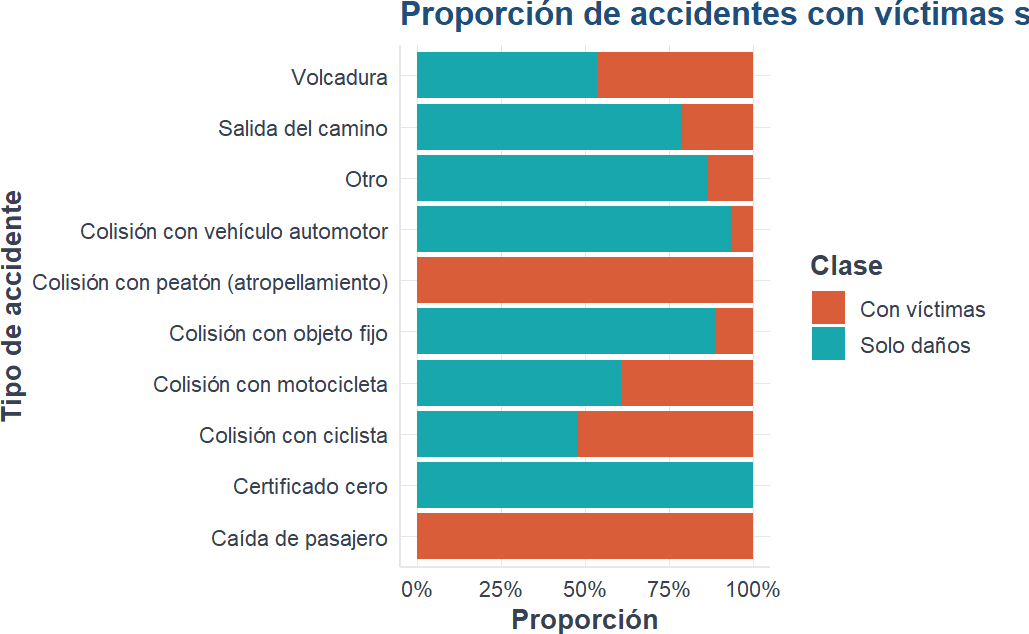
\includegraphics[width=0.92\linewidth,height=\textheight,keepaspectratio]{03-analisis-exploratorio_files/figure-pdf/proporcion-tipo-1.png}

\begin{tcolorbox}[enhanced jigsaw, arc=.35mm, bottomrule=.15mm, bottomtitle=1mm, breakable, colback=white, colbacktitle=quarto-callout-tip-color!10!white, colframe=quarto-callout-tip-color-frame, coltitle=black, left=2mm, leftrule=.75mm, opacityback=0, opacitybacktitle=0.6, rightrule=.15mm, title=\textcolor{quarto-callout-tip-color}{\faLightbulb}\hspace{0.5em}{Interpretación del resultado}, titlerule=0mm, toprule=.15mm, toptitle=1mm]

Esta gráfica compara proporciones, no cantidades absolutas. Permite
identificar tipos de accidente con mayor presencia relativa de víctimas.

\end{tcolorbox}

\section{Conclusión}\label{conclusiuxf3n-1}

El análisis exploratorio permite detectar patrones iniciales, revisar el
desbalance de clases e identificar variables útiles para modelar.

\bookmarksetup{startatroot}

\chapter{Regresión logística para
clasificación}\label{regresiuxf3n-loguxedstica-para-clasificaciuxf3n}

\section{Objetivos del capítulo}\label{objetivos-del-capuxedtulo-3}

Al finalizar este capítulo, el lector será capaz de ajustar una
regresión logística, predecir probabilidades y evaluar el desempeño.

\section{Fundamento matemático}\label{fundamento-matemuxe1tico}

La regresión logística utiliza la función:

\[
p = \frac{1}{1 + e^{-z}}
\]

donde (z = \beta\_0 + \beta\_1x\_1 + \cdots + \beta\_px\_p).

\section{Visualización de la función
logística}\label{visualizaciuxf3n-de-la-funciuxf3n-loguxedstica}

\begin{Shaded}
\begin{Highlighting}[]
\FunctionTok{library}\NormalTok{(ggplot2)}
\FunctionTok{source}\NormalTok{(}\StringTok{"util\_graficas.R"}\NormalTok{)}

\NormalTok{z }\OtherTok{\textless{}{-}} \FunctionTok{seq}\NormalTok{(}\SpecialCharTok{{-}}\DecValTok{10}\NormalTok{, }\DecValTok{10}\NormalTok{, }\AttributeTok{length.out =} \DecValTok{200}\NormalTok{)}
\NormalTok{datos\_logistica }\OtherTok{\textless{}{-}} \FunctionTok{data.frame}\NormalTok{(}\AttributeTok{z =}\NormalTok{ z, }\AttributeTok{p =} \DecValTok{1} \SpecialCharTok{/}\NormalTok{ (}\DecValTok{1} \SpecialCharTok{+} \FunctionTok{exp}\NormalTok{(}\SpecialCharTok{{-}}\NormalTok{z)))}

\FunctionTok{ggplot}\NormalTok{(datos\_logistica, }\FunctionTok{aes}\NormalTok{(}\AttributeTok{x =}\NormalTok{ z, }\AttributeTok{y =}\NormalTok{ p)) }\SpecialCharTok{+}
  \FunctionTok{geom\_line}\NormalTok{(}\AttributeTok{linewidth =} \FloatTok{1.2}\NormalTok{, }\AttributeTok{color =}\NormalTok{ col\_azul) }\SpecialCharTok{+}
  \FunctionTok{labs}\NormalTok{(}
    \AttributeTok{title =} \StringTok{"Función logística"}\NormalTok{,}
    \AttributeTok{subtitle =} \StringTok{"Transforma valores reales en probabilidades"}\NormalTok{,}
    \AttributeTok{x =} \StringTok{"z"}\NormalTok{,}
    \AttributeTok{y =} \StringTok{"Probabilidad"}
\NormalTok{  ) }\SpecialCharTok{+}
  \FunctionTok{tema\_libro}\NormalTok{()}
\end{Highlighting}
\end{Shaded}

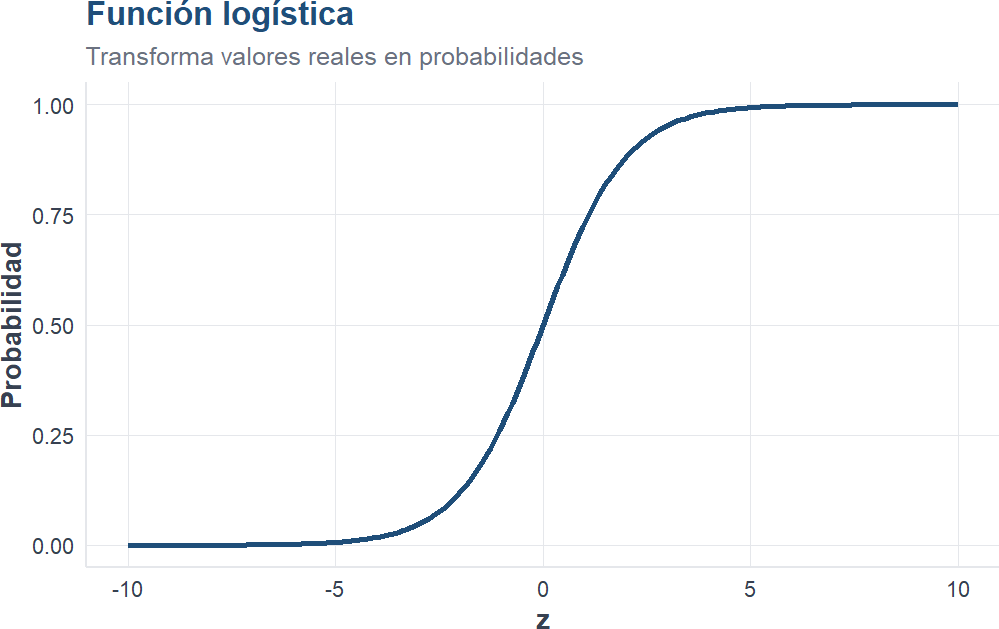
\includegraphics[width=0.92\linewidth,height=\textheight,keepaspectratio]{04-regresion-logistica_files/figure-pdf/grafica-logistica-1.png}

\begin{tcolorbox}[enhanced jigsaw, arc=.35mm, bottomrule=.15mm, bottomtitle=1mm, breakable, colback=white, colbacktitle=quarto-callout-note-color!10!white, colframe=quarto-callout-note-color-frame, coltitle=black, left=2mm, leftrule=.75mm, opacityback=0, opacitybacktitle=0.6, rightrule=.15mm, title=\textcolor{quarto-callout-note-color}{\faInfo}\hspace{0.5em}{Explicación del código}, titlerule=0mm, toprule=.15mm, toptitle=1mm]

Se genera una secuencia de valores para (z) y se calcula su probabilidad
usando la función logística.

\end{tcolorbox}

\begin{tcolorbox}[enhanced jigsaw, arc=.35mm, bottomrule=.15mm, bottomtitle=1mm, breakable, colback=white, colbacktitle=quarto-callout-tip-color!10!white, colframe=quarto-callout-tip-color-frame, coltitle=black, left=2mm, leftrule=.75mm, opacityback=0, opacitybacktitle=0.6, rightrule=.15mm, title=\textcolor{quarto-callout-tip-color}{\faLightbulb}\hspace{0.5em}{Interpretación del resultado}, titlerule=0mm, toprule=.15mm, toptitle=1mm]

La curva tiene forma de S. Valores negativos producen probabilidades
cercanas a cero y valores positivos probabilidades cercanas a uno.

\end{tcolorbox}

\section{Cargar paquetes y datos}\label{cargar-paquetes-y-datos}

\begin{Shaded}
\begin{Highlighting}[]
\FunctionTok{library}\NormalTok{(readr)}
\FunctionTok{library}\NormalTok{(dplyr)}
\FunctionTok{source}\NormalTok{(}\StringTok{"util\_graficas.R"}\NormalTok{)}

\NormalTok{ruta\_atus\_ml }\OtherTok{\textless{}{-}} \StringTok{"datos/atus\_ml\_preparado.csv"}

\ControlFlowTok{if}\NormalTok{ (}\FunctionTok{file.exists}\NormalTok{(ruta\_atus\_ml)) \{}
\NormalTok{  atus\_ml }\OtherTok{\textless{}{-}} \FunctionTok{read\_csv}\NormalTok{(ruta\_atus\_ml, }\AttributeTok{show\_col\_types =} \ConstantTok{FALSE}\NormalTok{)}
  \FunctionTok{print}\NormalTok{(}\StringTok{"Base preparada cargada correctamente."}\NormalTok{)}
\NormalTok{\} }\ControlFlowTok{else}\NormalTok{ \{}
\NormalTok{  atus\_ml }\OtherTok{\textless{}{-}} \ConstantTok{NULL}
  \FunctionTok{print}\NormalTok{(}\StringTok{"No se encontró el archivo datos/atus\_ml\_preparado.csv. Ejecuta primero el capítulo 2."}\NormalTok{)}
\NormalTok{\}}
\end{Highlighting}
\end{Shaded}

\begin{verbatim}
[1] "Base preparada cargada correctamente."
\end{verbatim}

\section{Preparar y dividir datos}\label{preparar-y-dividir-datos}

\begin{Shaded}
\begin{Highlighting}[]
\ControlFlowTok{if}\NormalTok{ (}\SpecialCharTok{!}\FunctionTok{is.null}\NormalTok{(atus\_ml)) \{}
\NormalTok{  atus\_modelo }\OtherTok{\textless{}{-}}\NormalTok{ atus\_ml }\SpecialCharTok{|\textgreater{}}
    \FunctionTok{mutate}\NormalTok{(}
      \AttributeTok{victimas\_binaria =} \FunctionTok{ifelse}\NormalTok{(accidente\_con\_victimas }\SpecialCharTok{==} \StringTok{"Con víctimas"}\NormalTok{, }\DecValTok{1}\NormalTok{, }\DecValTok{0}\NormalTok{),}
      \AttributeTok{MES =} \FunctionTok{as.factor}\NormalTok{(MES),}
      \AttributeTok{ID\_HORA =} \FunctionTok{as.numeric}\NormalTok{(ID\_HORA),}
      \AttributeTok{DIASEMANA =} \FunctionTok{as.factor}\NormalTok{(DIASEMANA),}
      \AttributeTok{TIPACCID =} \FunctionTok{as.factor}\NormalTok{(TIPACCID),}
      \AttributeTok{CAUSAACCI =} \FunctionTok{as.factor}\NormalTok{(CAUSAACCI),}
      \AttributeTok{accidente\_con\_victimas =} \FunctionTok{factor}\NormalTok{(accidente\_con\_victimas, }\AttributeTok{levels =} \FunctionTok{c}\NormalTok{(}\StringTok{"Con víctimas"}\NormalTok{, }\StringTok{"Solo daños"}\NormalTok{))}
\NormalTok{    )}

  \FunctionTok{set.seed}\NormalTok{(}\DecValTok{123}\NormalTok{)}
\NormalTok{  idx }\OtherTok{\textless{}{-}} \FunctionTok{sample}\NormalTok{(}\DecValTok{1}\SpecialCharTok{:}\FunctionTok{nrow}\NormalTok{(atus\_modelo), }\AttributeTok{size =} \FunctionTok{round}\NormalTok{(}\FloatTok{0.7} \SpecialCharTok{*} \FunctionTok{nrow}\NormalTok{(atus\_modelo)))}
\NormalTok{  entrenamiento }\OtherTok{\textless{}{-}}\NormalTok{ atus\_modelo[idx, ]}
\NormalTok{  prueba }\OtherTok{\textless{}{-}}\NormalTok{ atus\_modelo[}\SpecialCharTok{{-}}\NormalTok{idx, ]}
\NormalTok{\}}
\end{Highlighting}
\end{Shaded}

\begin{tcolorbox}[enhanced jigsaw, arc=.35mm, bottomrule=.15mm, bottomtitle=1mm, breakable, colback=white, colbacktitle=quarto-callout-note-color!10!white, colframe=quarto-callout-note-color-frame, coltitle=black, left=2mm, leftrule=.75mm, opacityback=0, opacitybacktitle=0.6, rightrule=.15mm, title=\textcolor{quarto-callout-note-color}{\faInfo}\hspace{0.5em}{Explicación del código}, titlerule=0mm, toprule=.15mm, toptitle=1mm]

La variable respuesta se transforma a binaria y la base se divide en
entrenamiento y prueba.

\end{tcolorbox}

\section{Ajustar modelo}\label{ajustar-modelo}

\begin{Shaded}
\begin{Highlighting}[]
\ControlFlowTok{if}\NormalTok{ (}\FunctionTok{exists}\NormalTok{(}\StringTok{"entrenamiento"}\NormalTok{)) \{}
\NormalTok{  modelo\_logistico }\OtherTok{\textless{}{-}} \FunctionTok{glm}\NormalTok{(}
\NormalTok{    victimas\_binaria }\SpecialCharTok{\textasciitilde{}}\NormalTok{ MES }\SpecialCharTok{+}\NormalTok{ ID\_HORA }\SpecialCharTok{+}\NormalTok{ DIASEMANA }\SpecialCharTok{+}\NormalTok{ TIPACCID }\SpecialCharTok{+}\NormalTok{ CAUSAACCI,}
    \AttributeTok{data =}\NormalTok{ entrenamiento,}
    \AttributeTok{family =}\NormalTok{ binomial}
\NormalTok{  )}

  \FunctionTok{head}\NormalTok{(}\FunctionTok{summary}\NormalTok{(modelo\_logistico)}\SpecialCharTok{$}\NormalTok{coefficients, }\DecValTok{12}\NormalTok{)}
\NormalTok{\}}
\end{Highlighting}
\end{Shaded}

\begin{verbatim}
                Estimate   Std. Error     z value     Pr(>|z|)
(Intercept) 18.107257168 101.84719297  0.17778848 8.588891e-01
MES02       -0.045765700   0.02975556 -1.53805548 1.240350e-01
MES03       -0.032191364   0.02927313 -1.09968980 2.714673e-01
MES04       -0.002838049   0.02945462 -0.09635327 9.232400e-01
MES05       -0.015408552   0.02906672 -0.53010979 5.960358e-01
MES06       -0.054753129   0.02983667 -1.83509526 6.649158e-02
MES07       -0.076296781   0.03035194 -2.51373620 1.194598e-02
MES08       -0.094049541   0.02997105 -3.13801278 1.700975e-03
MES09       -0.077109438   0.03015044 -2.55748998 1.054306e-02
MES10       -0.154152374   0.02979697 -5.17342485 2.298416e-07
MES11       -0.106385033   0.02950811 -3.60528073 3.118157e-04
MES12       -0.111888509   0.02959338 -3.78086333 1.562855e-04
\end{verbatim}

\begin{tcolorbox}[enhanced jigsaw, arc=.35mm, bottomrule=.15mm, bottomtitle=1mm, breakable, colback=white, colbacktitle=quarto-callout-tip-color!10!white, colframe=quarto-callout-tip-color-frame, coltitle=black, left=2mm, leftrule=.75mm, opacityback=0, opacitybacktitle=0.6, rightrule=.15mm, title=\textcolor{quarto-callout-tip-color}{\faLightbulb}\hspace{0.5em}{Interpretación del resultado}, titlerule=0mm, toprule=.15mm, toptitle=1mm]

Los coeficientes estiman el efecto de cada variable sobre el logit de la
probabilidad de accidente con víctimas.

\end{tcolorbox}

\section{Predicción y matriz de
confusión}\label{predicciuxf3n-y-matriz-de-confusiuxf3n}

\begin{Shaded}
\begin{Highlighting}[]
\ControlFlowTok{if}\NormalTok{ (}\FunctionTok{exists}\NormalTok{(}\StringTok{"modelo\_logistico"}\NormalTok{)) \{}
\NormalTok{  prueba}\SpecialCharTok{$}\NormalTok{probabilidad\_victimas }\OtherTok{\textless{}{-}} \FunctionTok{predict}\NormalTok{(modelo\_logistico, }\AttributeTok{newdata =}\NormalTok{ prueba, }\AttributeTok{type =} \StringTok{"response"}\NormalTok{)}
\NormalTok{  prueba}\SpecialCharTok{$}\NormalTok{prediccion\_03 }\OtherTok{\textless{}{-}} \FunctionTok{factor}\NormalTok{(}
    \FunctionTok{ifelse}\NormalTok{(prueba}\SpecialCharTok{$}\NormalTok{probabilidad\_victimas }\SpecialCharTok{\textgreater{}=} \FloatTok{0.3}\NormalTok{, }\StringTok{"Con víctimas"}\NormalTok{, }\StringTok{"Solo daños"}\NormalTok{),}
    \AttributeTok{levels =} \FunctionTok{c}\NormalTok{(}\StringTok{"Con víctimas"}\NormalTok{, }\StringTok{"Solo daños"}\NormalTok{)}
\NormalTok{  )}

\NormalTok{  matriz\_confusion\_03 }\OtherTok{\textless{}{-}} \FunctionTok{table}\NormalTok{(}
    \AttributeTok{Real =}\NormalTok{ prueba}\SpecialCharTok{$}\NormalTok{accidente\_con\_victimas,}
    \AttributeTok{Predicho =}\NormalTok{ prueba}\SpecialCharTok{$}\NormalTok{prediccion\_03}
\NormalTok{  )}

\NormalTok{  matriz\_confusion\_03}
\NormalTok{\}}
\end{Highlighting}
\end{Shaded}

\begin{verbatim}
              Predicho
Real           Con víctimas Solo daños
  Con víctimas        13765       6739
  Solo daños          14302      82382
\end{verbatim}

\begin{tcolorbox}[enhanced jigsaw, arc=.35mm, bottomrule=.15mm, bottomtitle=1mm, breakable, colback=white, colbacktitle=quarto-callout-note-color!10!white, colframe=quarto-callout-note-color-frame, coltitle=black, left=2mm, leftrule=.75mm, opacityback=0, opacitybacktitle=0.6, rightrule=.15mm, title=\textcolor{quarto-callout-note-color}{\faInfo}\hspace{0.5em}{Explicación del código}, titlerule=0mm, toprule=.15mm, toptitle=1mm]

Las probabilidades se convierten en clases usando un punto de corte de
0.3.

\end{tcolorbox}

\section{Métricas}\label{muxe9tricas}

\begin{Shaded}
\begin{Highlighting}[]
\ControlFlowTok{if}\NormalTok{ (}\FunctionTok{exists}\NormalTok{(}\StringTok{"matriz\_confusion\_03"}\NormalTok{)) \{}
\NormalTok{  VP }\OtherTok{\textless{}{-}}\NormalTok{ matriz\_confusion\_03[}\StringTok{"Con víctimas"}\NormalTok{, }\StringTok{"Con víctimas"}\NormalTok{]}
\NormalTok{  FN }\OtherTok{\textless{}{-}}\NormalTok{ matriz\_confusion\_03[}\StringTok{"Con víctimas"}\NormalTok{, }\StringTok{"Solo daños"}\NormalTok{]}
\NormalTok{  FP }\OtherTok{\textless{}{-}}\NormalTok{ matriz\_confusion\_03[}\StringTok{"Solo daños"}\NormalTok{, }\StringTok{"Con víctimas"}\NormalTok{]}
\NormalTok{  VN }\OtherTok{\textless{}{-}}\NormalTok{ matriz\_confusion\_03[}\StringTok{"Solo daños"}\NormalTok{, }\StringTok{"Solo daños"}\NormalTok{]}

  \FunctionTok{data.frame}\NormalTok{(}
    \AttributeTok{exactitud =}\NormalTok{ (VP }\SpecialCharTok{+}\NormalTok{ VN) }\SpecialCharTok{/}\NormalTok{ (VP }\SpecialCharTok{+}\NormalTok{ FN }\SpecialCharTok{+}\NormalTok{ FP }\SpecialCharTok{+}\NormalTok{ VN),}
    \AttributeTok{sensibilidad =}\NormalTok{ VP }\SpecialCharTok{/}\NormalTok{ (VP }\SpecialCharTok{+}\NormalTok{ FN),}
    \AttributeTok{especificidad =}\NormalTok{ VN }\SpecialCharTok{/}\NormalTok{ (VN }\SpecialCharTok{+}\NormalTok{ FP)}
\NormalTok{  )}
\NormalTok{\}}
\end{Highlighting}
\end{Shaded}

\begin{verbatim}
  exactitud sensibilidad especificidad
1 0.8204509    0.6713324     0.8520748
\end{verbatim}

\begin{tcolorbox}[enhanced jigsaw, arc=.35mm, bottomrule=.15mm, bottomtitle=1mm, breakable, colback=white, colbacktitle=quarto-callout-tip-color!10!white, colframe=quarto-callout-tip-color-frame, coltitle=black, left=2mm, leftrule=.75mm, opacityback=0, opacitybacktitle=0.6, rightrule=.15mm, title=\textcolor{quarto-callout-tip-color}{\faLightbulb}\hspace{0.5em}{Interpretación del resultado}, titlerule=0mm, toprule=.15mm, toptitle=1mm]

La sensibilidad mide la capacidad para detectar accidentes con víctimas;
la especificidad mide la capacidad para detectar accidentes de solo
daños.

\end{tcolorbox}

\section{Distribución de
probabilidades}\label{distribuciuxf3n-de-probabilidades}

\begin{Shaded}
\begin{Highlighting}[]
\ControlFlowTok{if}\NormalTok{ (}\FunctionTok{exists}\NormalTok{(}\StringTok{"prueba"}\NormalTok{)) \{}
  \FunctionTok{ggplot}\NormalTok{(prueba, }\FunctionTok{aes}\NormalTok{(}\AttributeTok{x =}\NormalTok{ probabilidad\_victimas, }\AttributeTok{fill =}\NormalTok{ accidente\_con\_victimas)) }\SpecialCharTok{+}
    \FunctionTok{geom\_histogram}\NormalTok{(}\AttributeTok{bins =} \DecValTok{30}\NormalTok{, }\AttributeTok{alpha =} \FloatTok{0.75}\NormalTok{, }\AttributeTok{position =} \StringTok{"identity"}\NormalTok{) }\SpecialCharTok{+}
    \FunctionTok{escala\_clases\_fill}\NormalTok{(}\AttributeTok{name =} \StringTok{"Clase real"}\NormalTok{) }\SpecialCharTok{+}
    \FunctionTok{labs}\NormalTok{(}
      \AttributeTok{title =} \StringTok{"Distribución de probabilidades predichas"}\NormalTok{,}
      \AttributeTok{subtitle =} \StringTok{"Regresión logística"}\NormalTok{,}
      \AttributeTok{x =} \StringTok{"Probabilidad predicha de accidente con víctimas"}\NormalTok{,}
      \AttributeTok{y =} \StringTok{"Frecuencia"}
\NormalTok{    ) }\SpecialCharTok{+}
    \FunctionTok{tema\_libro}\NormalTok{()}
\NormalTok{\}}
\end{Highlighting}
\end{Shaded}

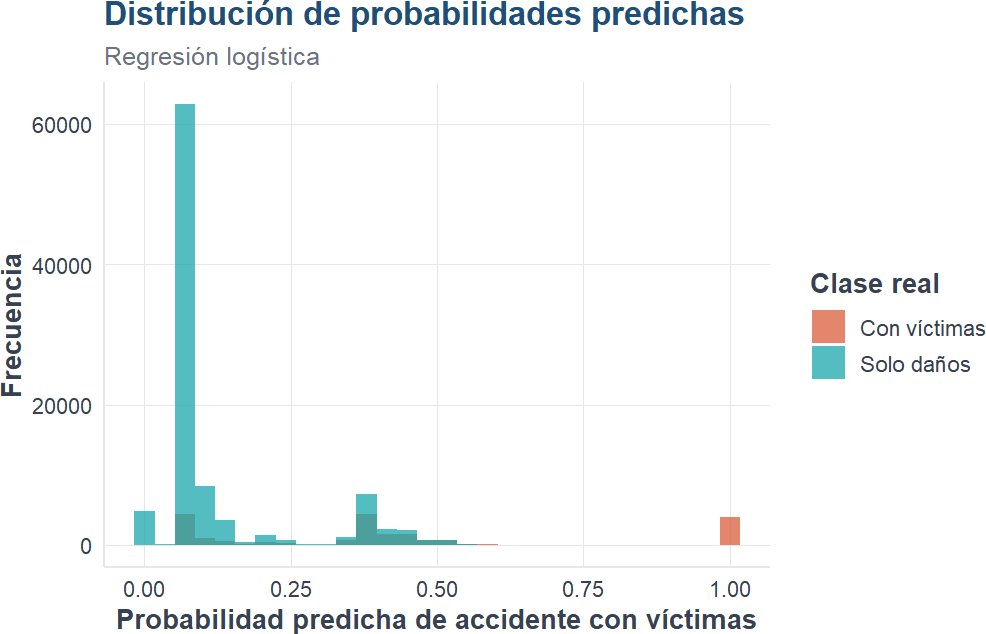
\includegraphics[width=0.92\linewidth,height=\textheight,keepaspectratio]{04-regresion-logistica_files/figure-pdf/histograma-logistica-1.png}

\section{Conclusión}\label{conclusiuxf3n-2}

La regresión logística es un modelo interpretable para clasificación
binaria. El punto de corte permite ajustar el balance entre sensibilidad
y especificidad.

\bookmarksetup{startatroot}

\chapter{k vecinos más cercanos,
k-NN}\label{k-vecinos-muxe1s-cercanos-k-nn}

\section{Objetivos del capítulo}\label{objetivos-del-capuxedtulo-4}

Al finalizar este capítulo, el lector será capaz de explicar k-NN,
preparar datos para este método, estandarizar variables y evaluar el
desempeño.

\section{Idea intuitiva}\label{idea-intuitiva}

k-NN clasifica una nueva observación según la clase más común entre sus
vecinos más cercanos.

\begin{Shaded}
\begin{Highlighting}[]
\FunctionTok{library}\NormalTok{(ggplot2)}
\FunctionTok{library}\NormalTok{(class)}
\FunctionTok{library}\NormalTok{(dplyr)}
\FunctionTok{library}\NormalTok{(tidyr)}
\FunctionTok{library}\NormalTok{(readr)}
\FunctionTok{source}\NormalTok{(}\StringTok{"util\_graficas.R"}\NormalTok{)}

\NormalTok{datos\_ejemplo }\OtherTok{\textless{}{-}} \FunctionTok{data.frame}\NormalTok{(}
  \AttributeTok{hora =} \FunctionTok{c}\NormalTok{(}\DecValTok{8}\NormalTok{, }\DecValTok{9}\NormalTok{, }\DecValTok{10}\NormalTok{, }\DecValTok{18}\NormalTok{, }\DecValTok{19}\NormalTok{, }\DecValTok{20}\NormalTok{, }\DecValTok{22}\NormalTok{, }\DecValTok{23}\NormalTok{),}
  \AttributeTok{mes =} \FunctionTok{c}\NormalTok{(}\DecValTok{1}\NormalTok{, }\DecValTok{1}\NormalTok{, }\DecValTok{2}\NormalTok{, }\DecValTok{6}\NormalTok{, }\DecValTok{6}\NormalTok{, }\DecValTok{7}\NormalTok{, }\DecValTok{12}\NormalTok{, }\DecValTok{12}\NormalTok{),}
  \AttributeTok{clase =} \FunctionTok{c}\NormalTok{(}\StringTok{"Solo daños"}\NormalTok{, }\StringTok{"Solo daños"}\NormalTok{, }\StringTok{"Solo daños"}\NormalTok{, }\StringTok{"Con víctimas"}\NormalTok{, }\StringTok{"Con víctimas"}\NormalTok{, }\StringTok{"Con víctimas"}\NormalTok{, }\StringTok{"Con víctimas"}\NormalTok{, }\StringTok{"Con víctimas"}\NormalTok{)}
\NormalTok{)}

\FunctionTok{ggplot}\NormalTok{(datos\_ejemplo, }\FunctionTok{aes}\NormalTok{(}\AttributeTok{x =}\NormalTok{ hora, }\AttributeTok{y =}\NormalTok{ mes, }\AttributeTok{color =}\NormalTok{ clase)) }\SpecialCharTok{+}
  \FunctionTok{geom\_point}\NormalTok{(}\AttributeTok{size =} \DecValTok{4}\NormalTok{) }\SpecialCharTok{+}
  \FunctionTok{escala\_clases\_color}\NormalTok{() }\SpecialCharTok{+}
  \FunctionTok{labs}\NormalTok{(}\AttributeTok{title =} \StringTok{"Ejemplo intuitivo de k{-}NN"}\NormalTok{, }\AttributeTok{x =} \StringTok{"Hora"}\NormalTok{, }\AttributeTok{y =} \StringTok{"Mes"}\NormalTok{, }\AttributeTok{color =} \StringTok{"Clase"}\NormalTok{) }\SpecialCharTok{+}
  \FunctionTok{tema\_libro}\NormalTok{()}
\end{Highlighting}
\end{Shaded}

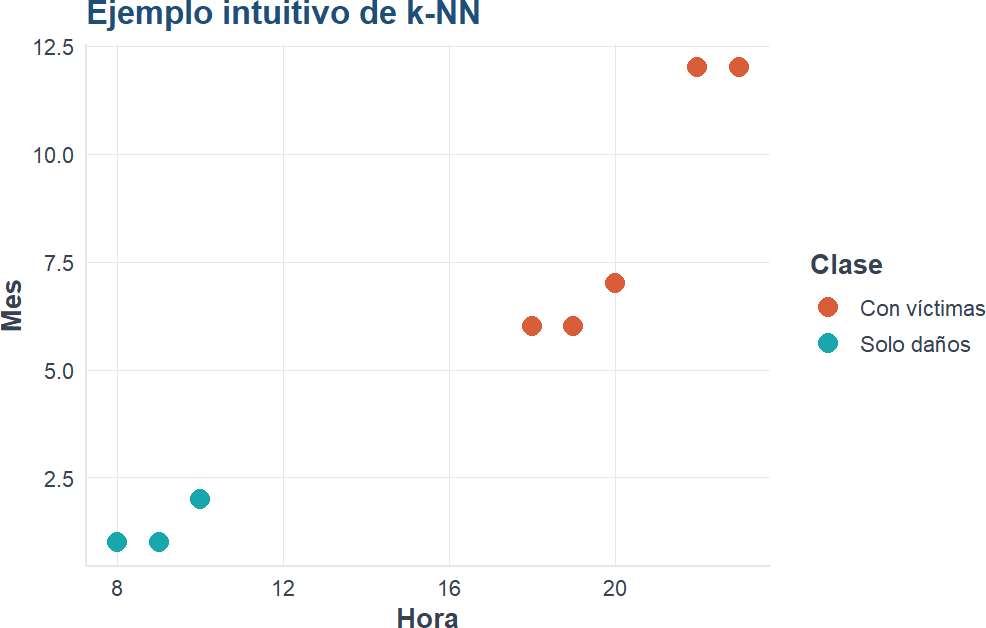
\includegraphics[width=0.92\linewidth,height=\textheight,keepaspectratio]{05-knn_files/figure-pdf/ejemplo-knn-1.png}

\begin{tcolorbox}[enhanced jigsaw, arc=.35mm, bottomrule=.15mm, bottomtitle=1mm, breakable, colback=white, colbacktitle=quarto-callout-note-color!10!white, colframe=quarto-callout-note-color-frame, coltitle=black, left=2mm, leftrule=.75mm, opacityback=0, opacitybacktitle=0.6, rightrule=.15mm, title=\textcolor{quarto-callout-note-color}{\faInfo}\hspace{0.5em}{Explicación del código}, titlerule=0mm, toprule=.15mm, toptitle=1mm]

Se construyen puntos artificiales para visualizar la idea de vecinos
cercanos.

\end{tcolorbox}

\section{Distancia euclidiana}\label{distancia-euclidiana}

\[
d(A,B) = \sqrt{(x_1-x_2)^2 + (y_1-y_2)^2}
\]

\begin{Shaded}
\begin{Highlighting}[]
\FunctionTok{sqrt}\NormalTok{((}\DecValTok{8} \SpecialCharTok{{-}} \DecValTok{10}\NormalTok{)}\SpecialCharTok{\^{}}\DecValTok{2} \SpecialCharTok{+}\NormalTok{ (}\DecValTok{1} \SpecialCharTok{{-}} \DecValTok{2}\NormalTok{)}\SpecialCharTok{\^{}}\DecValTok{2}\NormalTok{)}
\end{Highlighting}
\end{Shaded}

\begin{verbatim}
[1] 2.236068
\end{verbatim}

\begin{tcolorbox}[enhanced jigsaw, arc=.35mm, bottomrule=.15mm, bottomtitle=1mm, breakable, colback=white, colbacktitle=quarto-callout-tip-color!10!white, colframe=quarto-callout-tip-color-frame, coltitle=black, left=2mm, leftrule=.75mm, opacityback=0, opacitybacktitle=0.6, rightrule=.15mm, title=\textcolor{quarto-callout-tip-color}{\faLightbulb}\hspace{0.5em}{Interpretación del resultado}, titlerule=0mm, toprule=.15mm, toptitle=1mm]

Una distancia menor indica mayor similitud entre dos observaciones.

\end{tcolorbox}

\section{Cargar y preparar datos}\label{cargar-y-preparar-datos}

\begin{Shaded}
\begin{Highlighting}[]
\NormalTok{ruta\_atus\_ml }\OtherTok{\textless{}{-}} \StringTok{"datos/atus\_ml\_preparado.csv"}

\ControlFlowTok{if}\NormalTok{ (}\FunctionTok{file.exists}\NormalTok{(ruta\_atus\_ml)) \{}
\NormalTok{  atus\_ml }\OtherTok{\textless{}{-}} \FunctionTok{read\_csv}\NormalTok{(ruta\_atus\_ml, }\AttributeTok{show\_col\_types =} \ConstantTok{FALSE}\NormalTok{)}
  \FunctionTok{set.seed}\NormalTok{(}\DecValTok{123}\NormalTok{)}
\NormalTok{  atus\_knn\_base }\OtherTok{\textless{}{-}}\NormalTok{ atus\_ml }\SpecialCharTok{|\textgreater{}}
    \FunctionTok{sample\_n}\NormalTok{(}\FunctionTok{min}\NormalTok{(}\DecValTok{12000}\NormalTok{, }\FunctionTok{nrow}\NormalTok{(atus\_ml))) }\SpecialCharTok{|\textgreater{}}
    \FunctionTok{mutate}\NormalTok{(}
      \AttributeTok{accidente\_con\_victimas =} \FunctionTok{factor}\NormalTok{(accidente\_con\_victimas, }\AttributeTok{levels =} \FunctionTok{c}\NormalTok{(}\StringTok{"Con víctimas"}\NormalTok{, }\StringTok{"Solo daños"}\NormalTok{)),}
      \AttributeTok{MES =} \FunctionTok{as.factor}\NormalTok{(MES),}
      \AttributeTok{ID\_HORA =} \FunctionTok{as.numeric}\NormalTok{(ID\_HORA),}
      \AttributeTok{DIASEMANA =} \FunctionTok{as.factor}\NormalTok{(DIASEMANA),}
      \AttributeTok{TIPACCID =} \FunctionTok{as.factor}\NormalTok{(TIPACCID),}
      \AttributeTok{CAUSAACCI =} \FunctionTok{as.factor}\NormalTok{(CAUSAACCI)}
\NormalTok{    ) }\SpecialCharTok{|\textgreater{}}
    \FunctionTok{na.omit}\NormalTok{()}
\NormalTok{\}}
\end{Highlighting}
\end{Shaded}

\begin{tcolorbox}[enhanced jigsaw, arc=.35mm, bottomrule=.15mm, bottomtitle=1mm, breakable, colback=white, colbacktitle=quarto-callout-note-color!10!white, colframe=quarto-callout-note-color-frame, coltitle=black, left=2mm, leftrule=.75mm, opacityback=0, opacitybacktitle=0.6, rightrule=.15mm, title=\textcolor{quarto-callout-note-color}{\faInfo}\hspace{0.5em}{Explicación del código}, titlerule=0mm, toprule=.15mm, toptitle=1mm]

Se toma una muestra para que k-NN sea rápido y reproducible. Este método
puede ser costoso en bases grandes.

\end{tcolorbox}

\section{Modelo k-NN}\label{modelo-k-nn}

\begin{Shaded}
\begin{Highlighting}[]
\ControlFlowTok{if}\NormalTok{ (}\FunctionTok{exists}\NormalTok{(}\StringTok{"atus\_knn\_base"}\NormalTok{)) \{}
\NormalTok{  matriz\_predictoras }\OtherTok{\textless{}{-}} \FunctionTok{model.matrix}\NormalTok{(}\SpecialCharTok{\textasciitilde{}}\NormalTok{ ID\_HORA }\SpecialCharTok{+}\NormalTok{ MES }\SpecialCharTok{+}\NormalTok{ DIASEMANA }\SpecialCharTok{+}\NormalTok{ TIPACCID }\SpecialCharTok{+}\NormalTok{ CAUSAACCI }\SpecialCharTok{{-}} \DecValTok{1}\NormalTok{, }\AttributeTok{data =}\NormalTok{ atus\_knn\_base)}
\NormalTok{  y }\OtherTok{\textless{}{-}}\NormalTok{ atus\_knn\_base}\SpecialCharTok{$}\NormalTok{accidente\_con\_victimas}

  \FunctionTok{set.seed}\NormalTok{(}\DecValTok{123}\NormalTok{)}
\NormalTok{  idx }\OtherTok{\textless{}{-}} \FunctionTok{sample}\NormalTok{(}\DecValTok{1}\SpecialCharTok{:}\FunctionTok{nrow}\NormalTok{(matriz\_predictoras), }\AttributeTok{size =} \FunctionTok{round}\NormalTok{(}\FloatTok{0.7} \SpecialCharTok{*} \FunctionTok{nrow}\NormalTok{(matriz\_predictoras)))}
\NormalTok{  x\_entrenamiento }\OtherTok{\textless{}{-}}\NormalTok{ matriz\_predictoras[idx, ]}
\NormalTok{  x\_prueba }\OtherTok{\textless{}{-}}\NormalTok{ matriz\_predictoras[}\SpecialCharTok{{-}}\NormalTok{idx, ]}
\NormalTok{  y\_entrenamiento }\OtherTok{\textless{}{-}}\NormalTok{ y[idx]}
\NormalTok{  y\_prueba }\OtherTok{\textless{}{-}}\NormalTok{ y[}\SpecialCharTok{{-}}\NormalTok{idx]}

\NormalTok{  medias }\OtherTok{\textless{}{-}} \FunctionTok{apply}\NormalTok{(x\_entrenamiento, }\DecValTok{2}\NormalTok{, mean)}
\NormalTok{  desviaciones }\OtherTok{\textless{}{-}} \FunctionTok{apply}\NormalTok{(x\_entrenamiento, }\DecValTok{2}\NormalTok{, sd)}
\NormalTok{  desviaciones[desviaciones }\SpecialCharTok{==} \DecValTok{0}\NormalTok{] }\OtherTok{\textless{}{-}} \DecValTok{1}

\NormalTok{  x\_entrenamiento\_esc }\OtherTok{\textless{}{-}} \FunctionTok{scale}\NormalTok{(x\_entrenamiento, }\AttributeTok{center =}\NormalTok{ medias, }\AttributeTok{scale =}\NormalTok{ desviaciones)}
\NormalTok{  x\_prueba\_esc }\OtherTok{\textless{}{-}} \FunctionTok{scale}\NormalTok{(x\_prueba, }\AttributeTok{center =}\NormalTok{ medias, }\AttributeTok{scale =}\NormalTok{ desviaciones)}

\NormalTok{  pred\_knn\_5 }\OtherTok{\textless{}{-}} \FunctionTok{knn}\NormalTok{(x\_entrenamiento\_esc, x\_prueba\_esc, y\_entrenamiento, }\AttributeTok{k =} \DecValTok{5}\NormalTok{)}
  \FunctionTok{table}\NormalTok{(}\AttributeTok{Real =}\NormalTok{ y\_prueba, }\AttributeTok{Predicho =}\NormalTok{ pred\_knn\_5)}
\NormalTok{\}}
\end{Highlighting}
\end{Shaded}

\begin{verbatim}
              Predicho
Real           Con víctimas Solo daños
  Con víctimas          211        399
  Solo daños            144       2846
\end{verbatim}

\begin{tcolorbox}[enhanced jigsaw, arc=.35mm, bottomrule=.15mm, bottomtitle=1mm, breakable, colback=white, colbacktitle=quarto-callout-note-color!10!white, colframe=quarto-callout-note-color-frame, coltitle=black, left=2mm, leftrule=.75mm, opacityback=0, opacitybacktitle=0.6, rightrule=.15mm, title=\textcolor{quarto-callout-note-color}{\faInfo}\hspace{0.5em}{Explicación del código}, titlerule=0mm, toprule=.15mm, toptitle=1mm]

Se crean variables dummy, se estandarizan las columnas y se clasifica
con k igual a 5.

\end{tcolorbox}

\section{Comparación de valores de
k}\label{comparaciuxf3n-de-valores-de-k}

\begin{Shaded}
\begin{Highlighting}[]
\NormalTok{calcular\_metricas }\OtherTok{\textless{}{-}} \ControlFlowTok{function}\NormalTok{(real, predicho) \{}
\NormalTok{  real }\OtherTok{\textless{}{-}} \FunctionTok{factor}\NormalTok{(real, }\AttributeTok{levels =} \FunctionTok{c}\NormalTok{(}\StringTok{"Con víctimas"}\NormalTok{, }\StringTok{"Solo daños"}\NormalTok{))}
\NormalTok{  predicho }\OtherTok{\textless{}{-}} \FunctionTok{factor}\NormalTok{(predicho, }\AttributeTok{levels =} \FunctionTok{c}\NormalTok{(}\StringTok{"Con víctimas"}\NormalTok{, }\StringTok{"Solo daños"}\NormalTok{))}
\NormalTok{  m }\OtherTok{\textless{}{-}} \FunctionTok{table}\NormalTok{(}\AttributeTok{Real =}\NormalTok{ real, }\AttributeTok{Predicho =}\NormalTok{ predicho)}
\NormalTok{  VP }\OtherTok{\textless{}{-}}\NormalTok{ m[}\StringTok{"Con víctimas"}\NormalTok{, }\StringTok{"Con víctimas"}\NormalTok{]}
\NormalTok{  FN }\OtherTok{\textless{}{-}}\NormalTok{ m[}\StringTok{"Con víctimas"}\NormalTok{, }\StringTok{"Solo daños"}\NormalTok{]}
\NormalTok{  FP }\OtherTok{\textless{}{-}}\NormalTok{ m[}\StringTok{"Solo daños"}\NormalTok{, }\StringTok{"Con víctimas"}\NormalTok{]}
\NormalTok{  VN }\OtherTok{\textless{}{-}}\NormalTok{ m[}\StringTok{"Solo daños"}\NormalTok{, }\StringTok{"Solo daños"}\NormalTok{]}
  \FunctionTok{data.frame}\NormalTok{(}\AttributeTok{exactitud=}\NormalTok{(VP}\SpecialCharTok{+}\NormalTok{VN)}\SpecialCharTok{/}\NormalTok{(VP}\SpecialCharTok{+}\NormalTok{FN}\SpecialCharTok{+}\NormalTok{FP}\SpecialCharTok{+}\NormalTok{VN), }\AttributeTok{sensibilidad=}\NormalTok{VP}\SpecialCharTok{/}\NormalTok{(VP}\SpecialCharTok{+}\NormalTok{FN), }\AttributeTok{especificidad=}\NormalTok{VN}\SpecialCharTok{/}\NormalTok{(VN}\SpecialCharTok{+}\NormalTok{FP))}
\NormalTok{\}}

\ControlFlowTok{if}\NormalTok{ (}\FunctionTok{exists}\NormalTok{(}\StringTok{"x\_entrenamiento\_esc"}\NormalTok{)) \{}
\NormalTok{  valores\_k }\OtherTok{\textless{}{-}} \FunctionTok{c}\NormalTok{(}\DecValTok{3}\NormalTok{, }\DecValTok{5}\NormalTok{, }\DecValTok{11}\NormalTok{)}
\NormalTok{  resultados\_knn }\OtherTok{\textless{}{-}} \FunctionTok{data.frame}\NormalTok{()}

  \ControlFlowTok{for}\NormalTok{ (k\_actual }\ControlFlowTok{in}\NormalTok{ valores\_k) \{}
\NormalTok{    pred\_actual }\OtherTok{\textless{}{-}} \FunctionTok{knn}\NormalTok{(x\_entrenamiento\_esc, x\_prueba\_esc, y\_entrenamiento, }\AttributeTok{k =}\NormalTok{ k\_actual)}
\NormalTok{    tmp }\OtherTok{\textless{}{-}} \FunctionTok{calcular\_metricas}\NormalTok{(y\_prueba, pred\_actual)}
\NormalTok{    tmp}\SpecialCharTok{$}\NormalTok{k }\OtherTok{\textless{}{-}}\NormalTok{ k\_actual}
\NormalTok{    resultados\_knn }\OtherTok{\textless{}{-}} \FunctionTok{rbind}\NormalTok{(resultados\_knn, tmp)}
\NormalTok{  \}}

\NormalTok{  resultados\_knn }\OtherTok{\textless{}{-}}\NormalTok{ resultados\_knn }\SpecialCharTok{|\textgreater{}} \FunctionTok{select}\NormalTok{(k, exactitud, sensibilidad, especificidad)}
\NormalTok{  resultados\_knn}
\NormalTok{\}}
\end{Highlighting}
\end{Shaded}

\begin{verbatim}
   k exactitud sensibilidad especificidad
1  3 0.8433333    0.3770492     0.9384615
2  5 0.8480556    0.3491803     0.9498328
3 11 0.8558333    0.3377049     0.9615385
\end{verbatim}

\begin{Shaded}
\begin{Highlighting}[]
\ControlFlowTok{if}\NormalTok{ (}\FunctionTok{exists}\NormalTok{(}\StringTok{"resultados\_knn"}\NormalTok{)) \{}
\NormalTok{  resultados\_largos }\OtherTok{\textless{}{-}}\NormalTok{ resultados\_knn }\SpecialCharTok{|\textgreater{}}
    \FunctionTok{pivot\_longer}\NormalTok{(}\AttributeTok{cols =} \FunctionTok{c}\NormalTok{(exactitud, sensibilidad, especificidad), }\AttributeTok{names\_to =} \StringTok{"metrica"}\NormalTok{, }\AttributeTok{values\_to =} \StringTok{"valor"}\NormalTok{)}

  \FunctionTok{ggplot}\NormalTok{(resultados\_largos, }\FunctionTok{aes}\NormalTok{(}\AttributeTok{x =}\NormalTok{ k, }\AttributeTok{y =}\NormalTok{ valor, }\AttributeTok{color =}\NormalTok{ metrica, }\AttributeTok{group =}\NormalTok{ metrica)) }\SpecialCharTok{+}
    \FunctionTok{geom\_line}\NormalTok{(}\AttributeTok{linewidth =} \FloatTok{1.1}\NormalTok{) }\SpecialCharTok{+}
    \FunctionTok{geom\_point}\NormalTok{(}\AttributeTok{size =} \DecValTok{3}\NormalTok{) }\SpecialCharTok{+}
    \FunctionTok{scale\_color\_manual}\NormalTok{(}\AttributeTok{values =} \FunctionTok{c}\NormalTok{(}\AttributeTok{exactitud =}\NormalTok{ col\_azul, }\AttributeTok{sensibilidad =}\NormalTok{ col\_coral, }\AttributeTok{especificidad =}\NormalTok{ col\_turquesa)) }\SpecialCharTok{+}
    \FunctionTok{labs}\NormalTok{(}\AttributeTok{title =} \StringTok{"Comparación de métricas para distintos valores de k"}\NormalTok{, }\AttributeTok{x =} \StringTok{"Valor de k"}\NormalTok{, }\AttributeTok{y =} \StringTok{"Valor"}\NormalTok{) }\SpecialCharTok{+}
    \FunctionTok{tema\_libro}\NormalTok{()}
\NormalTok{\}}
\end{Highlighting}
\end{Shaded}

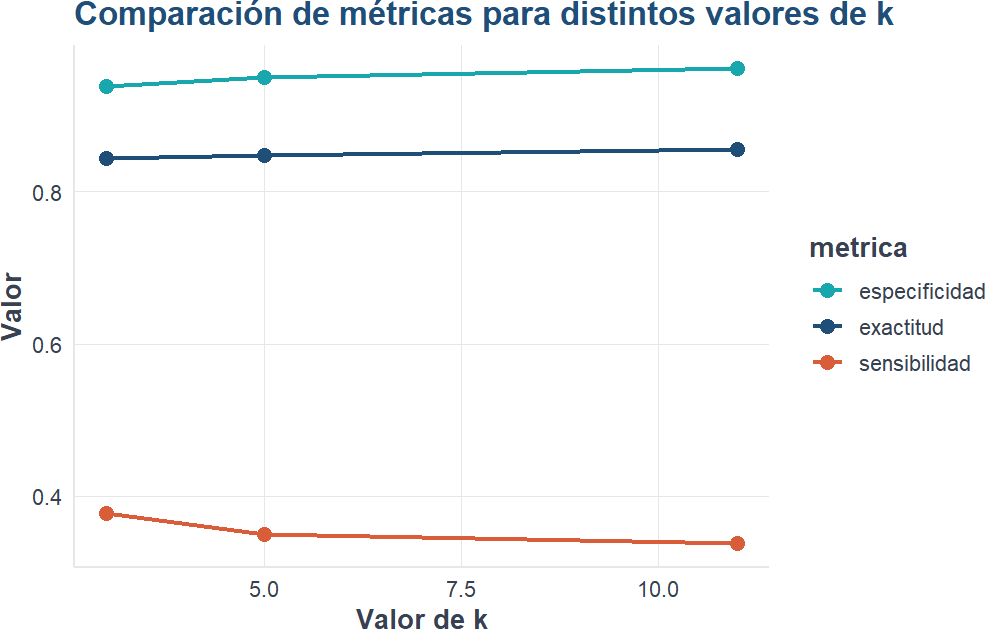
\includegraphics[width=0.92\linewidth,height=\textheight,keepaspectratio]{05-knn_files/figure-pdf/comparacion-knn-1.png}

\begin{tcolorbox}[enhanced jigsaw, arc=.35mm, bottomrule=.15mm, bottomtitle=1mm, breakable, colback=white, colbacktitle=quarto-callout-tip-color!10!white, colframe=quarto-callout-tip-color-frame, coltitle=black, left=2mm, leftrule=.75mm, opacityback=0, opacitybacktitle=0.6, rightrule=.15mm, title=\textcolor{quarto-callout-tip-color}{\faLightbulb}\hspace{0.5em}{Interpretación del resultado}, titlerule=0mm, toprule=.15mm, toptitle=1mm]

Cambiar k modifica el balance entre exactitud, sensibilidad y
especificidad. No existe un k universalmente mejor.

\end{tcolorbox}

\section{Conclusión}\label{conclusiuxf3n-3}

k-NN es un método intuitivo basado en similitud. Su desempeño depende
del valor de (k), del escalamiento y de la calidad de las variables
predictoras.

\bookmarksetup{startatroot}

\chapter{Árboles de decisión para
clasificación}\label{uxe1rboles-de-decisiuxf3n-para-clasificaciuxf3n}

\section{Objetivos del capítulo}\label{objetivos-del-capuxedtulo-5}

Al finalizar este capítulo, el lector será capaz de explicar la idea
básica de un árbol de decisión, entrenarlo en R y evaluar su desempeño.

\section{Introducción}\label{introducciuxf3n-2}

Los árboles de decisión clasifican observaciones mediante una secuencia
de preguntas. Son interpretables y pueden expresarse como reglas tipo
si-entonces.

\section{Fundamento matemático}\label{fundamento-matemuxe1tico-1}

Una medida común de impureza es el índice de Gini:

\[
Gini = 1 - \sum_{k=1}^{K} p_k^2
\]

\section{Cargar paquetes y datos}\label{cargar-paquetes-y-datos-1}

\begin{Shaded}
\begin{Highlighting}[]
\FunctionTok{library}\NormalTok{(readr)}
\FunctionTok{library}\NormalTok{(dplyr)}
\FunctionTok{library}\NormalTok{(rpart)}
\FunctionTok{source}\NormalTok{(}\StringTok{"util\_graficas.R"}\NormalTok{)}

\NormalTok{ruta\_atus\_ml }\OtherTok{\textless{}{-}} \StringTok{"datos/atus\_ml\_preparado.csv"}

\ControlFlowTok{if}\NormalTok{ (}\FunctionTok{file.exists}\NormalTok{(ruta\_atus\_ml)) \{}
\NormalTok{  atus\_ml }\OtherTok{\textless{}{-}} \FunctionTok{read\_csv}\NormalTok{(ruta\_atus\_ml, }\AttributeTok{show\_col\_types =} \ConstantTok{FALSE}\NormalTok{)}
  \FunctionTok{print}\NormalTok{(}\StringTok{"Base preparada cargada correctamente."}\NormalTok{)}
\NormalTok{\} }\ControlFlowTok{else}\NormalTok{ \{}
\NormalTok{  atus\_ml }\OtherTok{\textless{}{-}} \ConstantTok{NULL}
  \FunctionTok{print}\NormalTok{(}\StringTok{"No se encontró el archivo datos/atus\_ml\_preparado.csv. Ejecuta primero el capítulo 2."}\NormalTok{)}
\NormalTok{\}}
\end{Highlighting}
\end{Shaded}

\begin{verbatim}
[1] "Base preparada cargada correctamente."
\end{verbatim}

\section{Usar la base completa}\label{usar-la-base-completa}

\begin{Shaded}
\begin{Highlighting}[]
\ControlFlowTok{if}\NormalTok{ (}\SpecialCharTok{!}\FunctionTok{is.null}\NormalTok{(atus\_ml)) \{}
\NormalTok{  atus\_arbol\_base }\OtherTok{\textless{}{-}}\NormalTok{ atus\_ml }\SpecialCharTok{|\textgreater{}}
    \FunctionTok{mutate}\NormalTok{(}
      \AttributeTok{accidente\_con\_victimas =} \FunctionTok{factor}\NormalTok{(accidente\_con\_victimas, }\AttributeTok{levels =} \FunctionTok{c}\NormalTok{(}\StringTok{"Con víctimas"}\NormalTok{, }\StringTok{"Solo daños"}\NormalTok{)),}
      \AttributeTok{MES =} \FunctionTok{as.factor}\NormalTok{(MES),}
      \AttributeTok{ID\_HORA =} \FunctionTok{as.numeric}\NormalTok{(ID\_HORA),}
      \AttributeTok{DIASEMANA =} \FunctionTok{as.factor}\NormalTok{(DIASEMANA),}
      \AttributeTok{TIPACCID =} \FunctionTok{as.factor}\NormalTok{(TIPACCID),}
      \AttributeTok{CAUSAACCI =} \FunctionTok{as.factor}\NormalTok{(CAUSAACCI)}
\NormalTok{    ) }\SpecialCharTok{|\textgreater{}}
    \FunctionTok{na.omit}\NormalTok{()}

  \FunctionTok{data.frame}\NormalTok{(}\AttributeTok{filas =} \FunctionTok{nrow}\NormalTok{(atus\_arbol\_base), }\AttributeTok{columnas =} \FunctionTok{ncol}\NormalTok{(atus\_arbol\_base))}
\NormalTok{\}}
\end{Highlighting}
\end{Shaded}

\begin{verbatim}
   filas columnas
1 390627        6
\end{verbatim}

\begin{tcolorbox}[enhanced jigsaw, arc=.35mm, bottomrule=.15mm, bottomtitle=1mm, breakable, colback=white, colbacktitle=quarto-callout-note-color!10!white, colframe=quarto-callout-note-color-frame, coltitle=black, left=2mm, leftrule=.75mm, opacityback=0, opacitybacktitle=0.6, rightrule=.15mm, title=\textcolor{quarto-callout-note-color}{\faInfo}\hspace{0.5em}{Explicación del código}, titlerule=0mm, toprule=.15mm, toptitle=1mm]

Se usa la base completa, pero el crecimiento del árbol se controla
mediante parámetros del modelo.

\end{tcolorbox}

\section{División y entrenamiento}\label{divisiuxf3n-y-entrenamiento}

\begin{Shaded}
\begin{Highlighting}[]
\ControlFlowTok{if}\NormalTok{ (}\FunctionTok{exists}\NormalTok{(}\StringTok{"atus\_arbol\_base"}\NormalTok{)) \{}
  \FunctionTok{set.seed}\NormalTok{(}\DecValTok{123}\NormalTok{)}
\NormalTok{  idx }\OtherTok{\textless{}{-}} \FunctionTok{sample}\NormalTok{(}\DecValTok{1}\SpecialCharTok{:}\FunctionTok{nrow}\NormalTok{(atus\_arbol\_base), }\AttributeTok{size =} \FunctionTok{round}\NormalTok{(}\FloatTok{0.7} \SpecialCharTok{*} \FunctionTok{nrow}\NormalTok{(atus\_arbol\_base)))}
\NormalTok{  entrenamiento }\OtherTok{\textless{}{-}}\NormalTok{ atus\_arbol\_base[idx, ]}
\NormalTok{  prueba }\OtherTok{\textless{}{-}}\NormalTok{ atus\_arbol\_base[}\SpecialCharTok{{-}}\NormalTok{idx, ]}

\NormalTok{  modelo\_arbol }\OtherTok{\textless{}{-}} \FunctionTok{rpart}\NormalTok{(}
\NormalTok{    accidente\_con\_victimas }\SpecialCharTok{\textasciitilde{}}\NormalTok{ MES }\SpecialCharTok{+}\NormalTok{ ID\_HORA }\SpecialCharTok{+}\NormalTok{ DIASEMANA }\SpecialCharTok{+}\NormalTok{ TIPACCID }\SpecialCharTok{+}\NormalTok{ CAUSAACCI,}
    \AttributeTok{data =}\NormalTok{ entrenamiento,}
    \AttributeTok{method =} \StringTok{"class"}\NormalTok{,}
    \AttributeTok{control =} \FunctionTok{rpart.control}\NormalTok{(}\AttributeTok{cp =} \FloatTok{0.005}\NormalTok{, }\AttributeTok{minsplit =} \DecValTok{1000}\NormalTok{, }\AttributeTok{minbucket =} \DecValTok{300}\NormalTok{, }\AttributeTok{maxdepth =} \DecValTok{5}\NormalTok{)}
\NormalTok{  )}
\NormalTok{\}}
\end{Highlighting}
\end{Shaded}

\begin{tcolorbox}[enhanced jigsaw, arc=.35mm, bottomrule=.15mm, bottomtitle=1mm, breakable, colback=white, colbacktitle=quarto-callout-note-color!10!white, colframe=quarto-callout-note-color-frame, coltitle=black, left=2mm, leftrule=.75mm, opacityback=0, opacitybacktitle=0.6, rightrule=.15mm, title=\textcolor{quarto-callout-note-color}{\faInfo}\hspace{0.5em}{Explicación del código}, titlerule=0mm, toprule=.15mm, toptitle=1mm]

Se ajusta un árbol de decisión controlado para evitar sobreajuste y
salidas demasiado grandes.

\end{tcolorbox}

\section{Complejidad e importancia}\label{complejidad-e-importancia}

\begin{Shaded}
\begin{Highlighting}[]
\ControlFlowTok{if}\NormalTok{ (}\FunctionTok{exists}\NormalTok{(}\StringTok{"modelo\_arbol"}\NormalTok{)) }\FunctionTok{printcp}\NormalTok{(modelo\_arbol)}
\end{Highlighting}
\end{Shaded}

\begin{verbatim}

Classification tree:
rpart(formula = accidente_con_victimas ~ MES + ID_HORA + DIASEMANA + 
    TIPACCID + CAUSAACCI, data = entrenamiento, method = "class", 
    control = rpart.control(cp = 0.005, minsplit = 1000, minbucket = 300, 
        maxdepth = 5))

Variables actually used in tree construction:
[1] TIPACCID

Root node error: 47604/273439 = 0.17409

n= 273439 

        CP nsplit rel error xerror      xstd
1 0.097051      0    1.0000 1.0000 0.0041653
2 0.005000      2    0.8059 0.8059 0.0038150
\end{verbatim}

\begin{Shaded}
\begin{Highlighting}[]
\ControlFlowTok{if}\NormalTok{ (}\FunctionTok{exists}\NormalTok{(}\StringTok{"modelo\_arbol"}\NormalTok{)) \{}
\NormalTok{  importancia }\OtherTok{\textless{}{-}}\NormalTok{ modelo\_arbol}\SpecialCharTok{$}\NormalTok{variable.importance}
  \ControlFlowTok{if}\NormalTok{ (}\SpecialCharTok{!}\FunctionTok{is.null}\NormalTok{(importancia)) \{}
\NormalTok{    importancia\_df }\OtherTok{\textless{}{-}} \FunctionTok{data.frame}\NormalTok{(}\AttributeTok{variable =} \FunctionTok{names}\NormalTok{(importancia), }\AttributeTok{importancia =} \FunctionTok{as.numeric}\NormalTok{(importancia), }\AttributeTok{row.names =} \ConstantTok{NULL}\NormalTok{)}
\NormalTok{    importancia\_df }\OtherTok{\textless{}{-}}\NormalTok{ importancia\_df[}\FunctionTok{order}\NormalTok{(}\SpecialCharTok{{-}}\NormalTok{importancia\_df}\SpecialCharTok{$}\NormalTok{importancia), ]}
\NormalTok{    importancia\_df}
\NormalTok{  \}}
\NormalTok{\}}
\end{Highlighting}
\end{Shaded}

\begin{verbatim}
   variable importancia
1  TIPACCID   22919.330
2 CAUSAACCI    1093.984
\end{verbatim}

\begin{tcolorbox}[enhanced jigsaw, arc=.35mm, bottomrule=.15mm, bottomtitle=1mm, breakable, colback=white, colbacktitle=quarto-callout-tip-color!10!white, colframe=quarto-callout-tip-color-frame, coltitle=black, left=2mm, leftrule=.75mm, opacityback=0, opacitybacktitle=0.6, rightrule=.15mm, title=\textcolor{quarto-callout-tip-color}{\faLightbulb}\hspace{0.5em}{Interpretación del resultado}, titlerule=0mm, toprule=.15mm, toptitle=1mm]

La importancia de variables indica qué variables ayudan más a separar
accidentes con víctimas de accidentes de solo daños.

\end{tcolorbox}

\section{Gráfica opcional del
árbol}\label{gruxe1fica-opcional-del-uxe1rbol}

La gráfica completa del árbol puede ser pesada en PDF. El lector puede
ejecutarla manualmente en RStudio.

\begin{Shaded}
\begin{Highlighting}[]
\FunctionTok{plot}\NormalTok{(modelo\_arbol, }\AttributeTok{uniform =} \ConstantTok{TRUE}\NormalTok{, }\AttributeTok{margin =} \FloatTok{0.1}\NormalTok{)}
\FunctionTok{text}\NormalTok{(modelo\_arbol, }\AttributeTok{use.n =} \ConstantTok{TRUE}\NormalTok{, }\AttributeTok{cex =} \FloatTok{0.7}\NormalTok{)}
\end{Highlighting}
\end{Shaded}

\section{Predicción y métricas}\label{predicciuxf3n-y-muxe9tricas}

\begin{Shaded}
\begin{Highlighting}[]
\ControlFlowTok{if}\NormalTok{ (}\FunctionTok{exists}\NormalTok{(}\StringTok{"modelo\_arbol"}\NormalTok{)) \{}
\NormalTok{  pred\_arbol }\OtherTok{\textless{}{-}} \FunctionTok{predict}\NormalTok{(modelo\_arbol, }\AttributeTok{newdata =}\NormalTok{ prueba, }\AttributeTok{type =} \StringTok{"class"}\NormalTok{)}
\NormalTok{  real\_arbol }\OtherTok{\textless{}{-}} \FunctionTok{factor}\NormalTok{(prueba}\SpecialCharTok{$}\NormalTok{accidente\_con\_victimas, }\AttributeTok{levels =} \FunctionTok{c}\NormalTok{(}\StringTok{"Con víctimas"}\NormalTok{, }\StringTok{"Solo daños"}\NormalTok{))}
\NormalTok{  pred\_arbol }\OtherTok{\textless{}{-}} \FunctionTok{factor}\NormalTok{(pred\_arbol, }\AttributeTok{levels =} \FunctionTok{c}\NormalTok{(}\StringTok{"Con víctimas"}\NormalTok{, }\StringTok{"Solo daños"}\NormalTok{))}

\NormalTok{  matriz\_confusion\_arbol }\OtherTok{\textless{}{-}} \FunctionTok{table}\NormalTok{(}\AttributeTok{Real =}\NormalTok{ real\_arbol, }\AttributeTok{Predicho =}\NormalTok{ pred\_arbol)}
\NormalTok{  matriz\_confusion\_arbol}
\NormalTok{\}}
\end{Highlighting}
\end{Shaded}

\begin{verbatim}
              Predicho
Real           Con víctimas Solo daños
  Con víctimas         3965      16539
  Solo daños              0      96684
\end{verbatim}

\begin{Shaded}
\begin{Highlighting}[]
\ControlFlowTok{if}\NormalTok{ (}\FunctionTok{exists}\NormalTok{(}\StringTok{"matriz\_confusion\_arbol"}\NormalTok{)) \{}
\NormalTok{  VP }\OtherTok{\textless{}{-}}\NormalTok{ matriz\_confusion\_arbol[}\StringTok{"Con víctimas"}\NormalTok{, }\StringTok{"Con víctimas"}\NormalTok{]}
\NormalTok{  FN }\OtherTok{\textless{}{-}}\NormalTok{ matriz\_confusion\_arbol[}\StringTok{"Con víctimas"}\NormalTok{, }\StringTok{"Solo daños"}\NormalTok{]}
\NormalTok{  FP }\OtherTok{\textless{}{-}}\NormalTok{ matriz\_confusion\_arbol[}\StringTok{"Solo daños"}\NormalTok{, }\StringTok{"Con víctimas"}\NormalTok{]}
\NormalTok{  VN }\OtherTok{\textless{}{-}}\NormalTok{ matriz\_confusion\_arbol[}\StringTok{"Solo daños"}\NormalTok{, }\StringTok{"Solo daños"}\NormalTok{]}

  \FunctionTok{data.frame}\NormalTok{(}\AttributeTok{exactitud=}\NormalTok{(VP}\SpecialCharTok{+}\NormalTok{VN)}\SpecialCharTok{/}\NormalTok{(VP}\SpecialCharTok{+}\NormalTok{FN}\SpecialCharTok{+}\NormalTok{FP}\SpecialCharTok{+}\NormalTok{VN), }\AttributeTok{sensibilidad=}\NormalTok{VP}\SpecialCharTok{/}\NormalTok{(VP}\SpecialCharTok{+}\NormalTok{FN), }\AttributeTok{especificidad=}\NormalTok{VN}\SpecialCharTok{/}\NormalTok{(VN}\SpecialCharTok{+}\NormalTok{FP))}
\NormalTok{\}}
\end{Highlighting}
\end{Shaded}

\begin{verbatim}
  exactitud sensibilidad especificidad
1 0.8588678    0.1933769             1
\end{verbatim}

\begin{tcolorbox}[enhanced jigsaw, arc=.35mm, bottomrule=.15mm, bottomtitle=1mm, breakable, colback=white, colbacktitle=quarto-callout-tip-color!10!white, colframe=quarto-callout-tip-color-frame, coltitle=black, left=2mm, leftrule=.75mm, opacityback=0, opacitybacktitle=0.6, rightrule=.15mm, title=\textcolor{quarto-callout-tip-color}{\faLightbulb}\hspace{0.5em}{Interpretación del resultado}, titlerule=0mm, toprule=.15mm, toptitle=1mm]

La matriz de confusión y las métricas permiten evaluar el desempeño del
árbol sobre datos de prueba.

\end{tcolorbox}

\section{Conclusión}\label{conclusiuxf3n-4}

Los árboles de decisión son modelos intuitivos, visuales e
interpretables. Este capítulo prepara el camino para modelos basados en
muchos árboles, como Random Forest.

\bookmarksetup{startatroot}

\chapter{Random Forest para
clasificación}\label{random-forest-para-clasificaciuxf3n}

\section{Objetivos del capítulo}\label{objetivos-del-capuxedtulo-6}

Al finalizar este capítulo, el lector será capaz de explicar Random
Forest, entrenar un modelo en R, interpretar importancia de variables y
evaluar desempeño.

\section{Introducción}\label{introducciuxf3n-3}

Random Forest combina muchos árboles de decisión. Cada árbol aprende
sobre una muestra aleatoria de los datos y la predicción final se
obtiene por votación mayoritaria.

\section{Fundamento matemático}\label{fundamento-matemuxe1tico-2}

Si se construyen (B) árboles, la predicción final es:

\[
\hat{y}(x) = moda\{\hat{y}^{(1)}(x), \hat{y}^{(2)}(x), \ldots, \hat{y}^{(B)}(x)\}
\]

\section{Cargar paquetes y datos}\label{cargar-paquetes-y-datos-2}

\begin{Shaded}
\begin{Highlighting}[]
\FunctionTok{library}\NormalTok{(readr)}
\FunctionTok{library}\NormalTok{(dplyr)}
\FunctionTok{library}\NormalTok{(ggplot2)}
\FunctionTok{library}\NormalTok{(ranger)}
\FunctionTok{source}\NormalTok{(}\StringTok{"util\_graficas.R"}\NormalTok{)}

\NormalTok{ruta\_atus\_ml }\OtherTok{\textless{}{-}} \StringTok{"datos/atus\_ml\_preparado.csv"}

\ControlFlowTok{if}\NormalTok{ (}\FunctionTok{file.exists}\NormalTok{(ruta\_atus\_ml)) \{}
\NormalTok{  atus\_ml }\OtherTok{\textless{}{-}} \FunctionTok{read\_csv}\NormalTok{(ruta\_atus\_ml, }\AttributeTok{show\_col\_types =} \ConstantTok{FALSE}\NormalTok{)}
  \FunctionTok{print}\NormalTok{(}\StringTok{"Base preparada cargada correctamente."}\NormalTok{)}
\NormalTok{\} }\ControlFlowTok{else}\NormalTok{ \{}
\NormalTok{  atus\_ml }\OtherTok{\textless{}{-}} \ConstantTok{NULL}
  \FunctionTok{print}\NormalTok{(}\StringTok{"No se encontró el archivo datos/atus\_ml\_preparado.csv. Ejecuta primero el capítulo 2."}\NormalTok{)}
\NormalTok{\}}
\end{Highlighting}
\end{Shaded}

\begin{verbatim}
[1] "Base preparada cargada correctamente."
\end{verbatim}

\section{Muestra de trabajo}\label{muestra-de-trabajo}

\begin{Shaded}
\begin{Highlighting}[]
\ControlFlowTok{if}\NormalTok{ (}\SpecialCharTok{!}\FunctionTok{is.null}\NormalTok{(atus\_ml)) \{}
  \FunctionTok{set.seed}\NormalTok{(}\DecValTok{123}\NormalTok{)}
\NormalTok{  atus\_rf\_base }\OtherTok{\textless{}{-}}\NormalTok{ atus\_ml }\SpecialCharTok{|\textgreater{}}
    \FunctionTok{sample\_n}\NormalTok{(}\FunctionTok{min}\NormalTok{(}\DecValTok{30000}\NormalTok{, }\FunctionTok{nrow}\NormalTok{(atus\_ml))) }\SpecialCharTok{|\textgreater{}}
    \FunctionTok{mutate}\NormalTok{(}
      \AttributeTok{accidente\_con\_victimas =} \FunctionTok{factor}\NormalTok{(accidente\_con\_victimas, }\AttributeTok{levels =} \FunctionTok{c}\NormalTok{(}\StringTok{"Con víctimas"}\NormalTok{, }\StringTok{"Solo daños"}\NormalTok{)),}
      \AttributeTok{MES =} \FunctionTok{as.factor}\NormalTok{(MES),}
      \AttributeTok{ID\_HORA =} \FunctionTok{as.numeric}\NormalTok{(ID\_HORA),}
      \AttributeTok{DIASEMANA =} \FunctionTok{as.factor}\NormalTok{(DIASEMANA),}
      \AttributeTok{TIPACCID =} \FunctionTok{as.factor}\NormalTok{(TIPACCID),}
      \AttributeTok{CAUSAACCI =} \FunctionTok{as.factor}\NormalTok{(CAUSAACCI)}
\NormalTok{    ) }\SpecialCharTok{|\textgreater{}}
    \FunctionTok{na.omit}\NormalTok{()}

  \FunctionTok{data.frame}\NormalTok{(}\AttributeTok{filas =} \FunctionTok{nrow}\NormalTok{(atus\_rf\_base), }\AttributeTok{columnas =} \FunctionTok{ncol}\NormalTok{(atus\_rf\_base))}
\NormalTok{\}}
\end{Highlighting}
\end{Shaded}

\begin{verbatim}
  filas columnas
1 30000        6
\end{verbatim}

\begin{Shaded}
\begin{Highlighting}[]
\ControlFlowTok{if}\NormalTok{ (}\FunctionTok{exists}\NormalTok{(}\StringTok{"atus\_rf\_base"}\NormalTok{)) \{}
  \FunctionTok{ggplot}\NormalTok{(atus\_rf\_base, }\FunctionTok{aes}\NormalTok{(}\AttributeTok{x =}\NormalTok{ accidente\_con\_victimas, }\AttributeTok{fill =}\NormalTok{ accidente\_con\_victimas)) }\SpecialCharTok{+}
    \FunctionTok{geom\_bar}\NormalTok{(}\AttributeTok{width =} \FloatTok{0.7}\NormalTok{) }\SpecialCharTok{+}
    \FunctionTok{escala\_clases\_fill}\NormalTok{() }\SpecialCharTok{+}
    \FunctionTok{scale\_y\_continuous}\NormalTok{(}\AttributeTok{labels =}\NormalTok{ etiqueta\_numero) }\SpecialCharTok{+}
    \FunctionTok{labs}\NormalTok{(}
      \AttributeTok{title =} \StringTok{"Distribución de la variable respuesta"}\NormalTok{,}
      \AttributeTok{subtitle =} \StringTok{"Muestra para Random Forest"}\NormalTok{,}
      \AttributeTok{x =} \StringTok{"Clase"}\NormalTok{,}
      \AttributeTok{y =} \StringTok{"Número de accidentes"}
\NormalTok{    ) }\SpecialCharTok{+}
    \FunctionTok{tema\_libro}\NormalTok{() }\SpecialCharTok{+}
    \FunctionTok{theme}\NormalTok{(}\AttributeTok{legend.position =} \StringTok{"none"}\NormalTok{)}
\NormalTok{\}}
\end{Highlighting}
\end{Shaded}

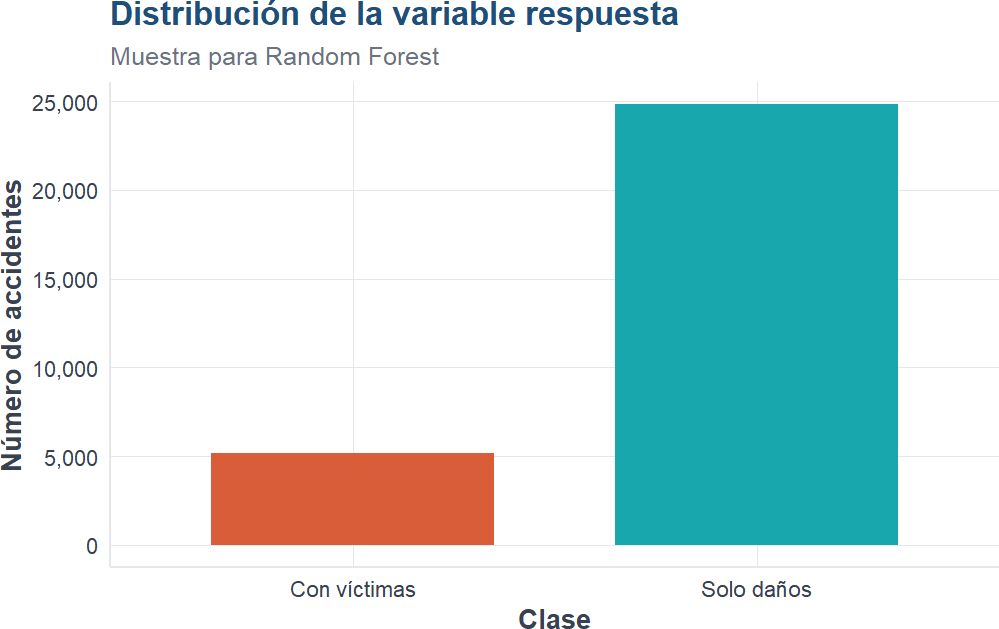
\includegraphics[width=0.92\linewidth,height=\textheight,keepaspectratio]{07-random-forest_files/figure-pdf/muestra-rf-1.png}

\begin{tcolorbox}[enhanced jigsaw, arc=.35mm, bottomrule=.15mm, bottomtitle=1mm, breakable, colback=white, colbacktitle=quarto-callout-note-color!10!white, colframe=quarto-callout-note-color-frame, coltitle=black, left=2mm, leftrule=.75mm, opacityback=0, opacitybacktitle=0.6, rightrule=.15mm, title=\textcolor{quarto-callout-note-color}{\faInfo}\hspace{0.5em}{Explicación del código}, titlerule=0mm, toprule=.15mm, toptitle=1mm]

Se toma una muestra de trabajo para mantener el tiempo de ejecución
razonable. El modelo Random Forest suele ser más pesado que un solo
árbol.

\end{tcolorbox}

\section{División en entrenamiento y
prueba}\label{divisiuxf3n-en-entrenamiento-y-prueba}

\begin{Shaded}
\begin{Highlighting}[]
\ControlFlowTok{if}\NormalTok{ (}\FunctionTok{exists}\NormalTok{(}\StringTok{"atus\_rf\_base"}\NormalTok{)) \{}
  \FunctionTok{set.seed}\NormalTok{(}\DecValTok{123}\NormalTok{)}
\NormalTok{  idx }\OtherTok{\textless{}{-}} \FunctionTok{sample}\NormalTok{(}\DecValTok{1}\SpecialCharTok{:}\FunctionTok{nrow}\NormalTok{(atus\_rf\_base), }\AttributeTok{size =} \FunctionTok{round}\NormalTok{(}\FloatTok{0.7} \SpecialCharTok{*} \FunctionTok{nrow}\NormalTok{(atus\_rf\_base)))}
\NormalTok{  entrenamiento }\OtherTok{\textless{}{-}}\NormalTok{ atus\_rf\_base[idx, ]}
\NormalTok{  prueba }\OtherTok{\textless{}{-}}\NormalTok{ atus\_rf\_base[}\SpecialCharTok{{-}}\NormalTok{idx, ]}

  \FunctionTok{data.frame}\NormalTok{(}\AttributeTok{conjunto =} \FunctionTok{c}\NormalTok{(}\StringTok{"Entrenamiento"}\NormalTok{, }\StringTok{"Prueba"}\NormalTok{), }\AttributeTok{registros =} \FunctionTok{c}\NormalTok{(}\FunctionTok{nrow}\NormalTok{(entrenamiento), }\FunctionTok{nrow}\NormalTok{(prueba)))}
\NormalTok{\}}
\end{Highlighting}
\end{Shaded}

\begin{verbatim}
       conjunto registros
1 Entrenamiento     21000
2        Prueba      9000
\end{verbatim}

\section{Ajustar Random Forest}\label{ajustar-random-forest}

\begin{Shaded}
\begin{Highlighting}[]
\ControlFlowTok{if}\NormalTok{ (}\FunctionTok{exists}\NormalTok{(}\StringTok{"entrenamiento"}\NormalTok{)) \{}
  \FunctionTok{set.seed}\NormalTok{(}\DecValTok{123}\NormalTok{)}

\NormalTok{  modelo\_rf }\OtherTok{\textless{}{-}} \FunctionTok{ranger}\NormalTok{(}
\NormalTok{    accidente\_con\_victimas }\SpecialCharTok{\textasciitilde{}}\NormalTok{ MES }\SpecialCharTok{+}\NormalTok{ ID\_HORA }\SpecialCharTok{+}\NormalTok{ DIASEMANA }\SpecialCharTok{+}\NormalTok{ TIPACCID }\SpecialCharTok{+}\NormalTok{ CAUSAACCI,}
    \AttributeTok{data =}\NormalTok{ entrenamiento,}
    \AttributeTok{num.trees =} \DecValTok{200}\NormalTok{,}
    \AttributeTok{mtry =} \DecValTok{3}\NormalTok{,}
    \AttributeTok{min.node.size =} \DecValTok{20}\NormalTok{,}
    \AttributeTok{importance =} \StringTok{"impurity"}\NormalTok{,}
    \AttributeTok{probability =} \ConstantTok{TRUE}\NormalTok{,}
    \AttributeTok{seed =} \DecValTok{123}
\NormalTok{  )}

\NormalTok{  modelo\_rf}
\NormalTok{\}}
\end{Highlighting}
\end{Shaded}

\begin{verbatim}
Ranger result

Call:
 ranger(accidente_con_victimas ~ MES + ID_HORA + DIASEMANA + TIPACCID +      CAUSAACCI, data = entrenamiento, num.trees = 200, mtry = 3,      min.node.size = 20, importance = "impurity", probability = TRUE,      seed = 123) 

Type:                             Probability estimation 
Number of trees:                  200 
Sample size:                      21000 
Number of independent variables:  5 
Mtry:                             3 
Target node size:                 20 
Variable importance mode:         impurity 
Splitrule:                        gini 
OOB prediction error (Brier s.):  0.1066668 
\end{verbatim}

\begin{tcolorbox}[enhanced jigsaw, arc=.35mm, bottomrule=.15mm, bottomtitle=1mm, breakable, colback=white, colbacktitle=quarto-callout-tip-color!10!white, colframe=quarto-callout-tip-color-frame, coltitle=black, left=2mm, leftrule=.75mm, opacityback=0, opacitybacktitle=0.6, rightrule=.15mm, title=\textcolor{quarto-callout-tip-color}{\faLightbulb}\hspace{0.5em}{Interpretación del resultado}, titlerule=0mm, toprule=.15mm, toptitle=1mm]

El resumen del modelo muestra cuántos árboles se construyeron, cuántas
variables se probaron en cada división y el error fuera de bolsa.

\end{tcolorbox}

\section{Importancia de variables}\label{importancia-de-variables}

\begin{Shaded}
\begin{Highlighting}[]
\ControlFlowTok{if}\NormalTok{ (}\FunctionTok{exists}\NormalTok{(}\StringTok{"modelo\_rf"}\NormalTok{)) \{}
\NormalTok{  importancia\_rf }\OtherTok{\textless{}{-}} \FunctionTok{data.frame}\NormalTok{(}
    \AttributeTok{variable =} \FunctionTok{names}\NormalTok{(modelo\_rf}\SpecialCharTok{$}\NormalTok{variable.importance),}
    \AttributeTok{importancia =} \FunctionTok{as.numeric}\NormalTok{(modelo\_rf}\SpecialCharTok{$}\NormalTok{variable.importance)}
\NormalTok{  ) }\SpecialCharTok{|\textgreater{}}
    \FunctionTok{arrange}\NormalTok{(}\FunctionTok{desc}\NormalTok{(importancia))}

\NormalTok{  importancia\_rf}
\NormalTok{\}}
\end{Highlighting}
\end{Shaded}

\begin{verbatim}
   variable importancia
1  TIPACCID   1608.8347
2   ID_HORA    416.7870
3       MES    324.9780
4 DIASEMANA    234.4944
5 CAUSAACCI    220.5923
\end{verbatim}

\begin{Shaded}
\begin{Highlighting}[]
\ControlFlowTok{if}\NormalTok{ (}\FunctionTok{exists}\NormalTok{(}\StringTok{"importancia\_rf"}\NormalTok{)) \{}
  \FunctionTok{ggplot}\NormalTok{(importancia\_rf, }\FunctionTok{aes}\NormalTok{(}\AttributeTok{x =} \FunctionTok{reorder}\NormalTok{(variable, importancia), }\AttributeTok{y =}\NormalTok{ importancia)) }\SpecialCharTok{+}
    \FunctionTok{geom\_col}\NormalTok{(}\AttributeTok{fill =}\NormalTok{ col\_azul, }\AttributeTok{width =} \FloatTok{0.75}\NormalTok{) }\SpecialCharTok{+}
    \FunctionTok{coord\_flip}\NormalTok{() }\SpecialCharTok{+}
    \FunctionTok{labs}\NormalTok{(}\AttributeTok{title =} \StringTok{"Importancia de variables en Random Forest"}\NormalTok{, }\AttributeTok{x =} \StringTok{"Variable"}\NormalTok{, }\AttributeTok{y =} \StringTok{"Importancia"}\NormalTok{) }\SpecialCharTok{+}
    \FunctionTok{tema\_libro}\NormalTok{()}
\NormalTok{\}}
\end{Highlighting}
\end{Shaded}

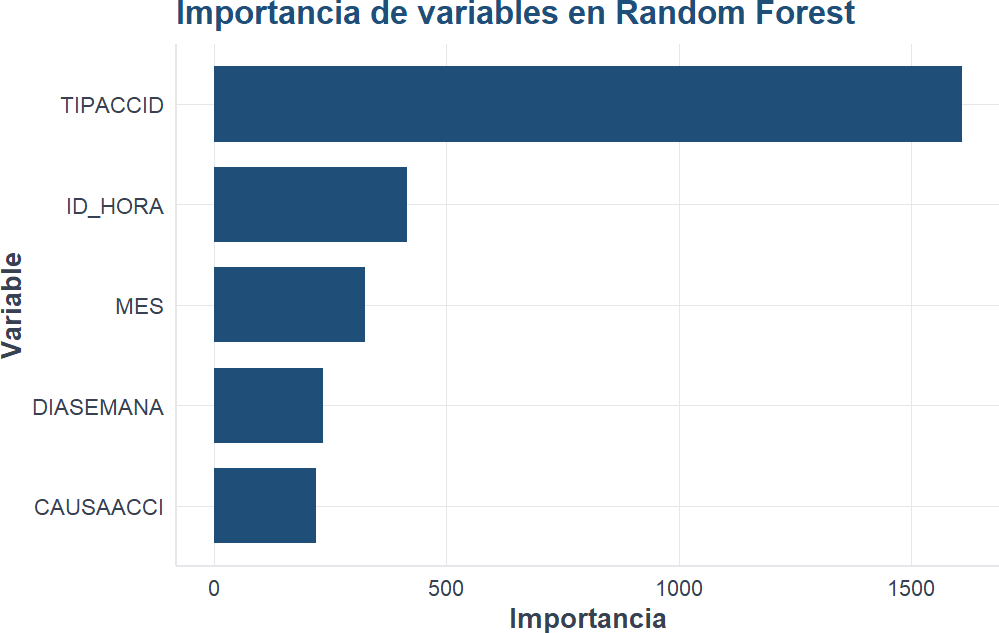
\includegraphics[width=0.92\linewidth,height=\textheight,keepaspectratio]{07-random-forest_files/figure-pdf/importancia-rf-1.png}

\begin{tcolorbox}[enhanced jigsaw, arc=.35mm, bottomrule=.15mm, bottomtitle=1mm, breakable, colback=white, colbacktitle=quarto-callout-note-color!10!white, colframe=quarto-callout-note-color-frame, coltitle=black, left=2mm, leftrule=.75mm, opacityback=0, opacitybacktitle=0.6, rightrule=.15mm, title=\textcolor{quarto-callout-note-color}{\faInfo}\hspace{0.5em}{Explicación del código}, titlerule=0mm, toprule=.15mm, toptitle=1mm]

La importancia de variables muestra qué predictores aportan más a la
reducción de impureza en los árboles del bosque.

\end{tcolorbox}

\section{Predicción y métricas}\label{predicciuxf3n-y-muxe9tricas-1}

\begin{Shaded}
\begin{Highlighting}[]
\ControlFlowTok{if}\NormalTok{ (}\FunctionTok{exists}\NormalTok{(}\StringTok{"modelo\_rf"}\NormalTok{)) \{}
\NormalTok{  predicciones\_rf }\OtherTok{\textless{}{-}} \FunctionTok{predict}\NormalTok{(modelo\_rf, }\AttributeTok{data =}\NormalTok{ prueba)}
\NormalTok{  probabilidades\_rf }\OtherTok{\textless{}{-}}\NormalTok{ predicciones\_rf}\SpecialCharTok{$}\NormalTok{predictions[, }\StringTok{"Con víctimas"}\NormalTok{]}
\NormalTok{  clases\_rf }\OtherTok{\textless{}{-}} \FunctionTok{colnames}\NormalTok{(predicciones\_rf}\SpecialCharTok{$}\NormalTok{predictions)[}\FunctionTok{max.col}\NormalTok{(predicciones\_rf}\SpecialCharTok{$}\NormalTok{predictions, }\AttributeTok{ties.method =} \StringTok{"first"}\NormalTok{)]}
\NormalTok{  clases\_rf }\OtherTok{\textless{}{-}} \FunctionTok{factor}\NormalTok{(clases\_rf, }\AttributeTok{levels =} \FunctionTok{c}\NormalTok{(}\StringTok{"Con víctimas"}\NormalTok{, }\StringTok{"Solo daños"}\NormalTok{))}
\NormalTok{  real\_rf }\OtherTok{\textless{}{-}} \FunctionTok{factor}\NormalTok{(prueba}\SpecialCharTok{$}\NormalTok{accidente\_con\_victimas, }\AttributeTok{levels =} \FunctionTok{c}\NormalTok{(}\StringTok{"Con víctimas"}\NormalTok{, }\StringTok{"Solo daños"}\NormalTok{))}

\NormalTok{  matriz\_confusion\_rf }\OtherTok{\textless{}{-}} \FunctionTok{table}\NormalTok{(}\AttributeTok{Real =}\NormalTok{ real\_rf, }\AttributeTok{Predicho =}\NormalTok{ clases\_rf)}
\NormalTok{  matriz\_confusion\_rf}
\NormalTok{\}}
\end{Highlighting}
\end{Shaded}

\begin{verbatim}
              Predicho
Real           Con víctimas Solo daños
  Con víctimas          475        991
  Solo daños            265       7269
\end{verbatim}

\begin{Shaded}
\begin{Highlighting}[]
\ControlFlowTok{if}\NormalTok{ (}\FunctionTok{exists}\NormalTok{(}\StringTok{"matriz\_confusion\_rf"}\NormalTok{)) \{}
\NormalTok{  VP }\OtherTok{\textless{}{-}}\NormalTok{ matriz\_confusion\_rf[}\StringTok{"Con víctimas"}\NormalTok{, }\StringTok{"Con víctimas"}\NormalTok{]}
\NormalTok{  FN }\OtherTok{\textless{}{-}}\NormalTok{ matriz\_confusion\_rf[}\StringTok{"Con víctimas"}\NormalTok{, }\StringTok{"Solo daños"}\NormalTok{]}
\NormalTok{  FP }\OtherTok{\textless{}{-}}\NormalTok{ matriz\_confusion\_rf[}\StringTok{"Solo daños"}\NormalTok{, }\StringTok{"Con víctimas"}\NormalTok{]}
\NormalTok{  VN }\OtherTok{\textless{}{-}}\NormalTok{ matriz\_confusion\_rf[}\StringTok{"Solo daños"}\NormalTok{, }\StringTok{"Solo daños"}\NormalTok{]}

  \FunctionTok{data.frame}\NormalTok{(}\AttributeTok{exactitud=}\NormalTok{(VP}\SpecialCharTok{+}\NormalTok{VN)}\SpecialCharTok{/}\NormalTok{(VP}\SpecialCharTok{+}\NormalTok{FN}\SpecialCharTok{+}\NormalTok{FP}\SpecialCharTok{+}\NormalTok{VN), }\AttributeTok{sensibilidad=}\NormalTok{VP}\SpecialCharTok{/}\NormalTok{(VP}\SpecialCharTok{+}\NormalTok{FN), }\AttributeTok{especificidad=}\NormalTok{VN}\SpecialCharTok{/}\NormalTok{(VN}\SpecialCharTok{+}\NormalTok{FP))}
\NormalTok{\}}
\end{Highlighting}
\end{Shaded}

\begin{verbatim}
  exactitud sensibilidad especificidad
1 0.8604444    0.3240109     0.9648261
\end{verbatim}

\begin{tcolorbox}[enhanced jigsaw, arc=.35mm, bottomrule=.15mm, bottomtitle=1mm, breakable, colback=white, colbacktitle=quarto-callout-tip-color!10!white, colframe=quarto-callout-tip-color-frame, coltitle=black, left=2mm, leftrule=.75mm, opacityback=0, opacitybacktitle=0.6, rightrule=.15mm, title=\textcolor{quarto-callout-tip-color}{\faLightbulb}\hspace{0.5em}{Interpretación del resultado}, titlerule=0mm, toprule=.15mm, toptitle=1mm]

La sensibilidad indica qué tan bien detecta accidentes con víctimas. La
especificidad indica qué tan bien reconoce accidentes de solo daños.

\end{tcolorbox}

\section{Distribución de probabilidades
predichas}\label{distribuciuxf3n-de-probabilidades-predichas}

\begin{Shaded}
\begin{Highlighting}[]
\ControlFlowTok{if}\NormalTok{ (}\FunctionTok{exists}\NormalTok{(}\StringTok{"probabilidades\_rf"}\NormalTok{)) \{}
\NormalTok{  datos\_prob\_rf }\OtherTok{\textless{}{-}} \FunctionTok{data.frame}\NormalTok{(}\AttributeTok{probabilidad =}\NormalTok{ probabilidades\_rf, }\AttributeTok{clase\_real =}\NormalTok{ real\_rf)}

  \FunctionTok{ggplot}\NormalTok{(datos\_prob\_rf, }\FunctionTok{aes}\NormalTok{(}\AttributeTok{x =}\NormalTok{ probabilidad, }\AttributeTok{fill =}\NormalTok{ clase\_real)) }\SpecialCharTok{+}
    \FunctionTok{geom\_histogram}\NormalTok{(}\AttributeTok{bins =} \DecValTok{30}\NormalTok{, }\AttributeTok{alpha =} \FloatTok{0.75}\NormalTok{, }\AttributeTok{position =} \StringTok{"identity"}\NormalTok{) }\SpecialCharTok{+}
    \FunctionTok{escala\_clases\_fill}\NormalTok{(}\AttributeTok{name =} \StringTok{"Clase real"}\NormalTok{) }\SpecialCharTok{+}
    \FunctionTok{labs}\NormalTok{(}
      \AttributeTok{title =} \StringTok{"Distribución de probabilidades predichas"}\NormalTok{,}
      \AttributeTok{subtitle =} \StringTok{"Random Forest"}\NormalTok{,}
      \AttributeTok{x =} \StringTok{"Probabilidad predicha de \textquotesingle{}Con víctimas\textquotesingle{}"}\NormalTok{,}
      \AttributeTok{y =} \StringTok{"Frecuencia"}
\NormalTok{    ) }\SpecialCharTok{+}
    \FunctionTok{tema\_libro}\NormalTok{()}
\NormalTok{\}}
\end{Highlighting}
\end{Shaded}

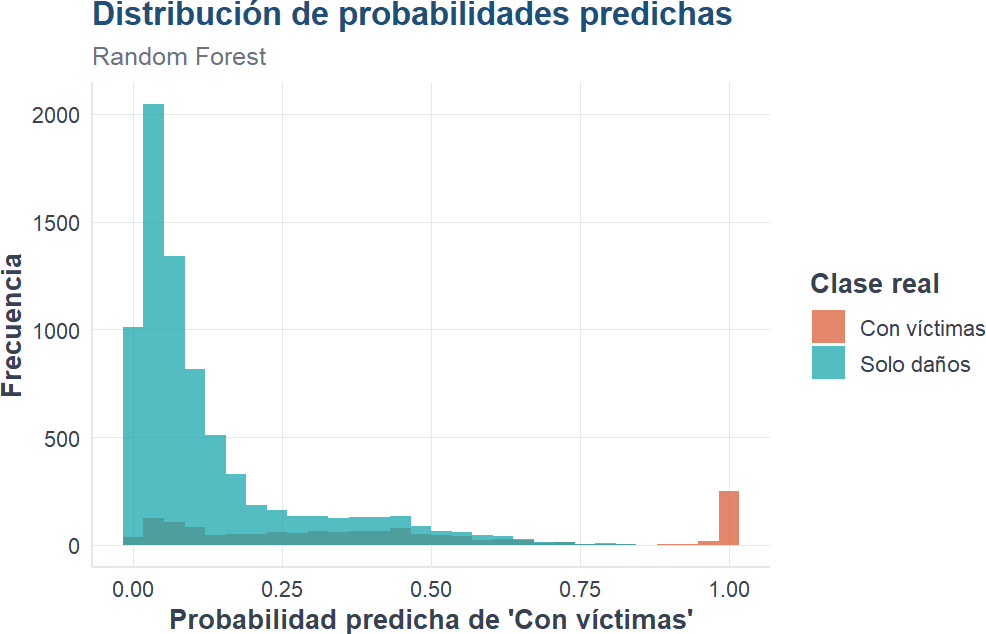
\includegraphics[width=0.92\linewidth,height=\textheight,keepaspectratio]{07-random-forest_files/figure-pdf/histograma-rf-1.png}

\section{Conclusión}\label{conclusiuxf3n-5}

Random Forest mejora la estabilidad y la capacidad predictiva de un solo
árbol al combinar muchos árboles. Es uno de los métodos más útiles para
clasificación aplicada.


\backmatter


\end{document}
